\subsection{Momentum Corrections}
\label{sec:momentum_corrections}
\subsubsection{Electron Corrections}
Due to imperfections in alignment, magnetic field mapping and other software reconstruction related effects the reconstructed momenta of final state particles may differ slightly from the true momenta. This can most readily be seen in the position of certain missing mass peaks e.g. the missing neutron peak in our exclusive channel e'(n)$\pi^+$. The peak should appear at precisely 0.8828~GeV$^2$ but due to these imperfections can appear shifted. We perform momentum corrections in a two stage process, first by developing momentum corrections for the electron using the position of the proton mass in elastic events and then secondly developing corrections for the $\pi^+$ after applying those electron corrections and fixing the position of the missing neutron peak in e'(n)$\pi^+$ events. The kinematic range of the elastic events does not extend to the full phase space of the exclusive $\pi^+$ final state electrons but as will be shown extrapolations are reasonably stable and the correction appears safe even in these regions.

The elastic sample is taken from the gmn train. Data are divided into four periods: Su22, Fa22 solenoid-1, Fa22 solenoid+1 and Sp23. As an example of the need for momentum corrections the position of the elastic peak in each of the six FD sectors of CLAS12 is shown in Fig.~\ref{fig:su22_uncorrected_elastic_peak}. Several sectors show comparatively large deviations from the expected peak value of W = 0.938~GeV. Additionally, possible $\theta$ dependence can be considered (although compared to earlier run groups, the $\theta$ and $\phi$ dependence of the missing mass peaks seem markedly improved, probably due to improvements in the pass-2 DC alignment procedures) and is shown in Fig.~\ref{fig:fa22_uncorrected_theta_trends}.

\begin{figure}[htp]
\internallinenumbers
\begin{subfigure}[t]{0.99\textwidth}
\centering
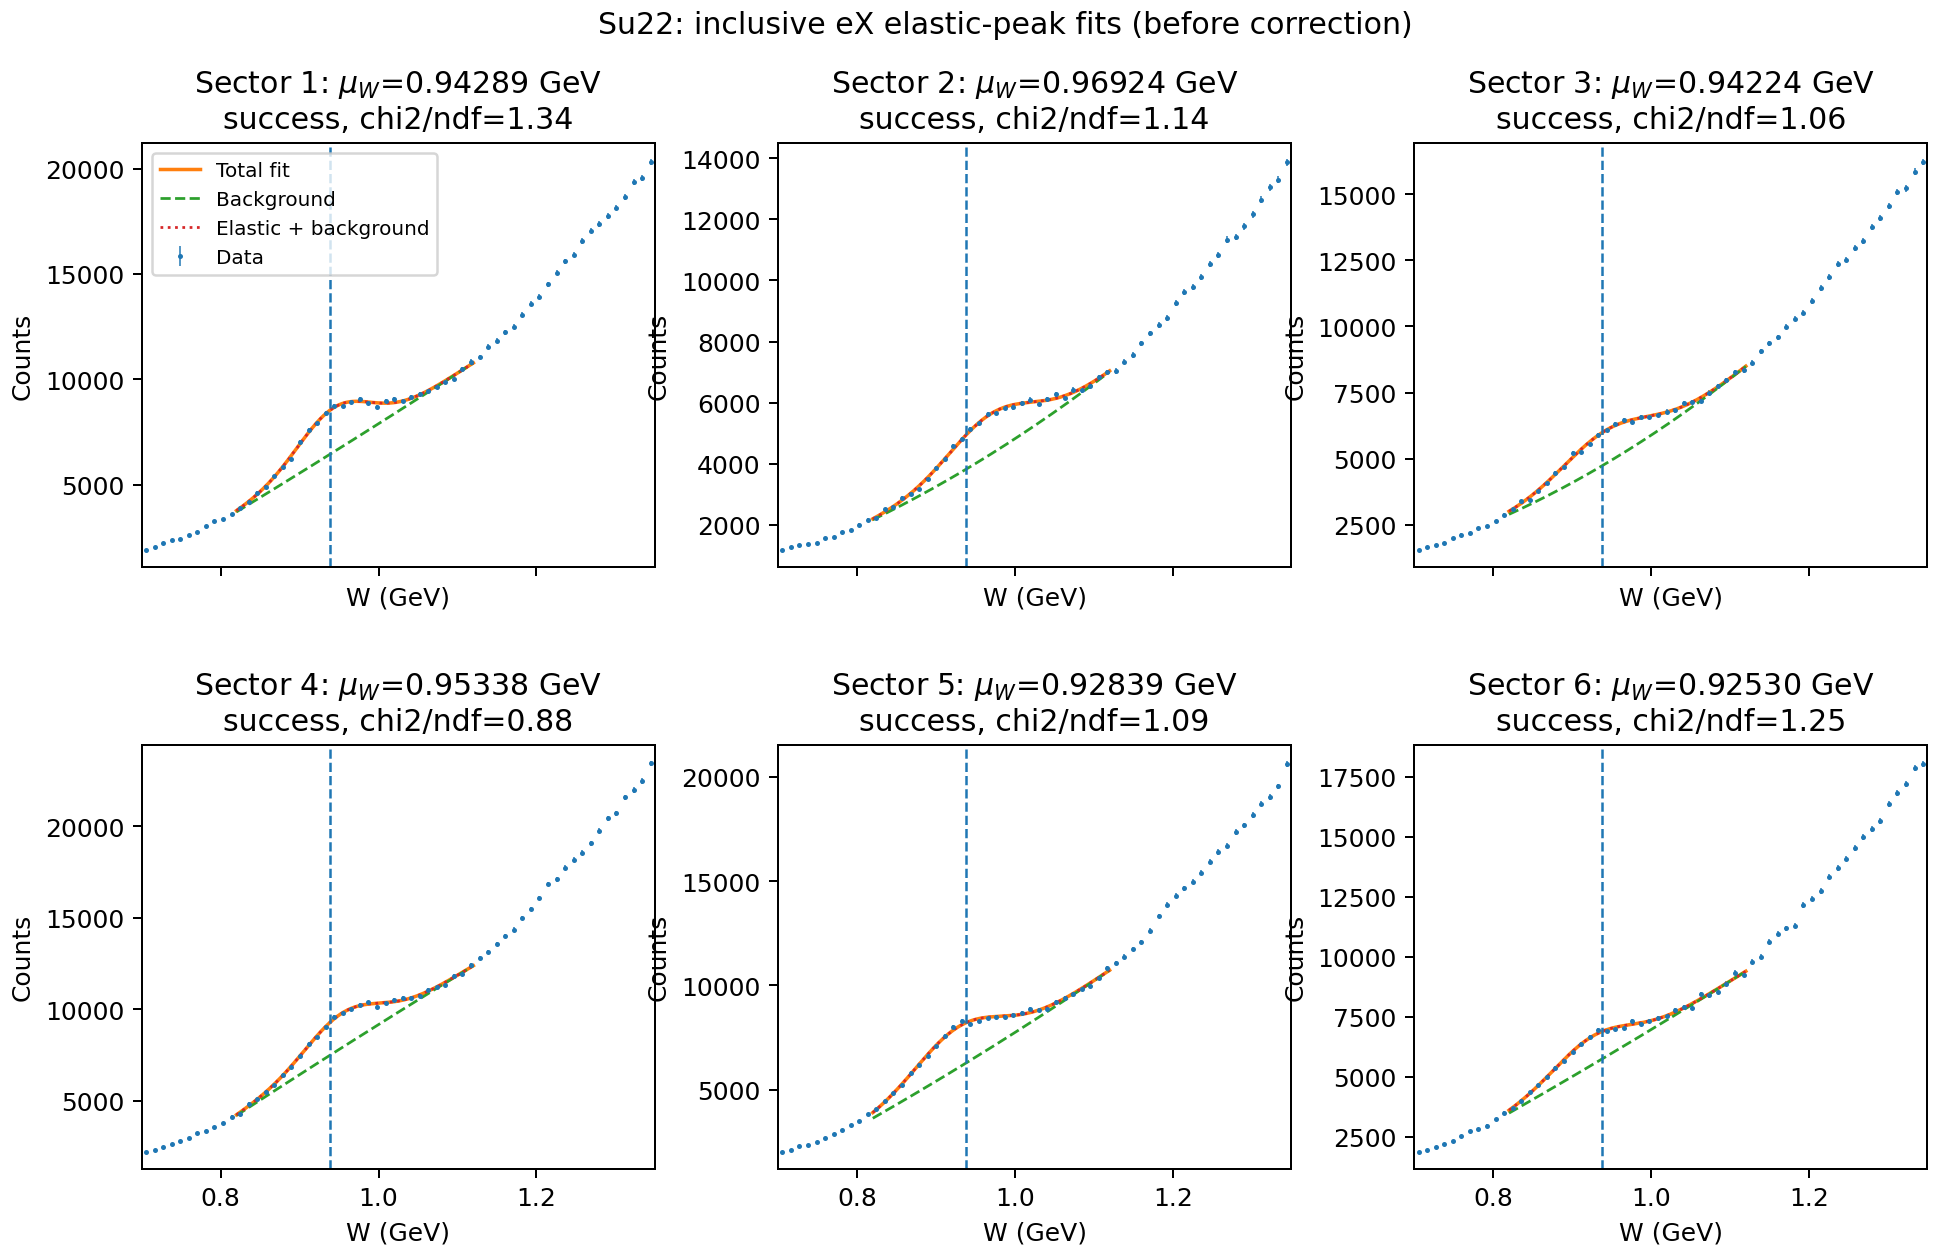
\includegraphics[width=\linewidth]{figures/channel_selection/momentum_corrections/electron/su22_integrated_w_by_sector.png}
\end{subfigure}
\caption{Elastic peak position in each of the six FD sectors of CLAS12 for Su22.} % Caption for the whole figure
\label{fig:su22_uncorrected_elastic_peak} % Label for referencing the entire figure
\end{figure}

\begin{figure}[htp]
\internallinenumbers
\begin{subfigure}[t]{0.99\textwidth}
\centering
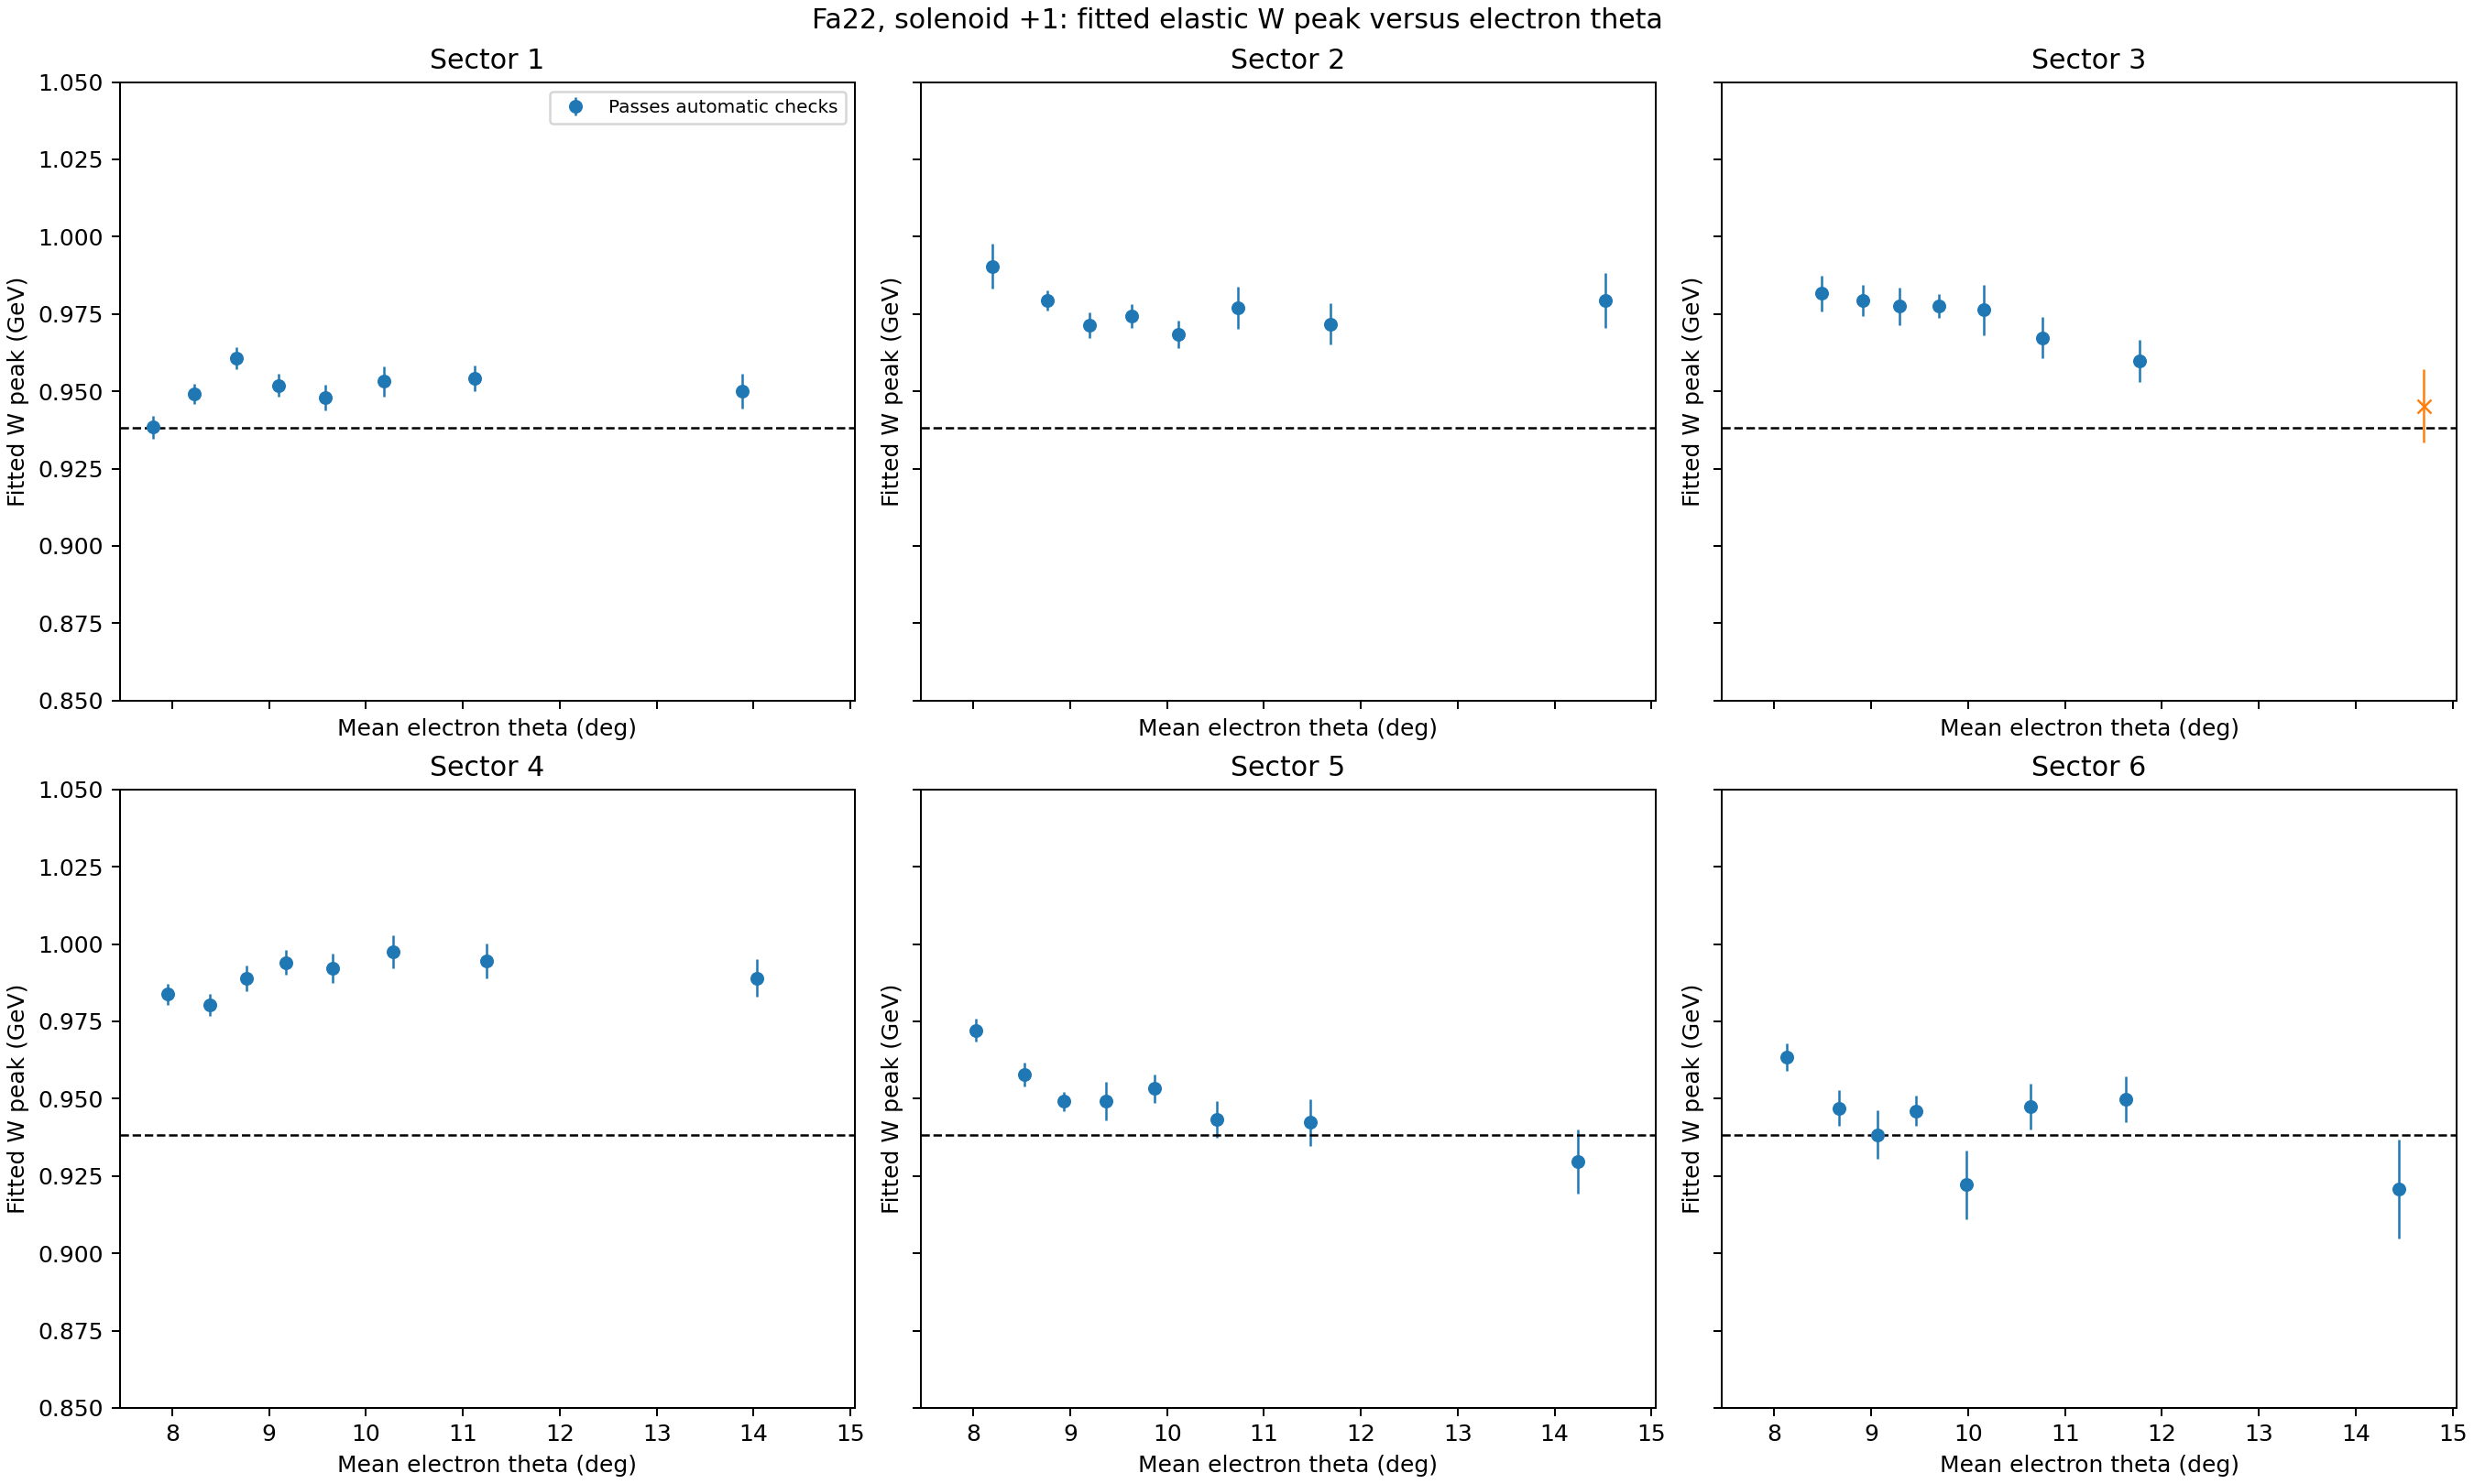
\includegraphics[width=\linewidth]{figures/channel_selection/momentum_corrections/electron/fa22_solenoid_plus_w_peak_vs_theta.png}
\end{subfigure}
\caption{Fitted elastic peak in each of the six FD sectors of CLAS12 as a function of $e_\theta$ for Fa22 solenoid-1.} % Caption for the whole figure
\label{fig:fa22_uncorrected_theta_trends}
\end{figure}

The $W$ spectrum is fit to a signal + background, $f(W) = S(W) + B(W)$ where the signal is a Gaussian,
\begin{align}
    S(W) = A e^{ \left[ - \frac{(W - \mu_W)^2}{2\sigma^2_W}\right]},
\end{align}
and the background is a simple quadratic polynomial,
\begin{align}
    B(W) = b_0 + b_1 W + b_2 W^2.
\end{align}
The measured momentum is assumed to differ from the true momentum by some small factor,
\begin{align}
    p_e^{\text{corr}} = (1+\delta) p_e,
\end{align}
with the $\delta$ fit to minimize the fitted elastic peak difference from the true elastic peak. The process is repeated in each $e_\theta$ bin and a simple polynomial is chosen for the $\delta(e_\theta)$,
\begin{align}
    \delta(e_\theta) = a_0 + a_1 e_\theta + a_2 e_\theta^2 + a_3 e_\theta^3 + ...
\end{align}
where the order of the polynomial is selected according to the Akaike Information Criterion (AIC) by requiring it to exceed 2 (to balance improved $\chi^2$ vs statistical fluctuations),
\begin{align}
    \text{AIC}_c = \chi^2 + 2k + \frac{2k(k+1)}{n-k-1},
\end{align}
where $n$ is the degree of the polynomial and $k$ is the number of fitted points. In general a linear function is preferred with a quadratic being used in some cases. An example of these fits can be seen in Fig.~\ref{fig:fa22_fitted_theta_trends}.

\begin{figure}[htp]
\internallinenumbers
\begin{subfigure}[t]{0.99\textwidth}
\centering
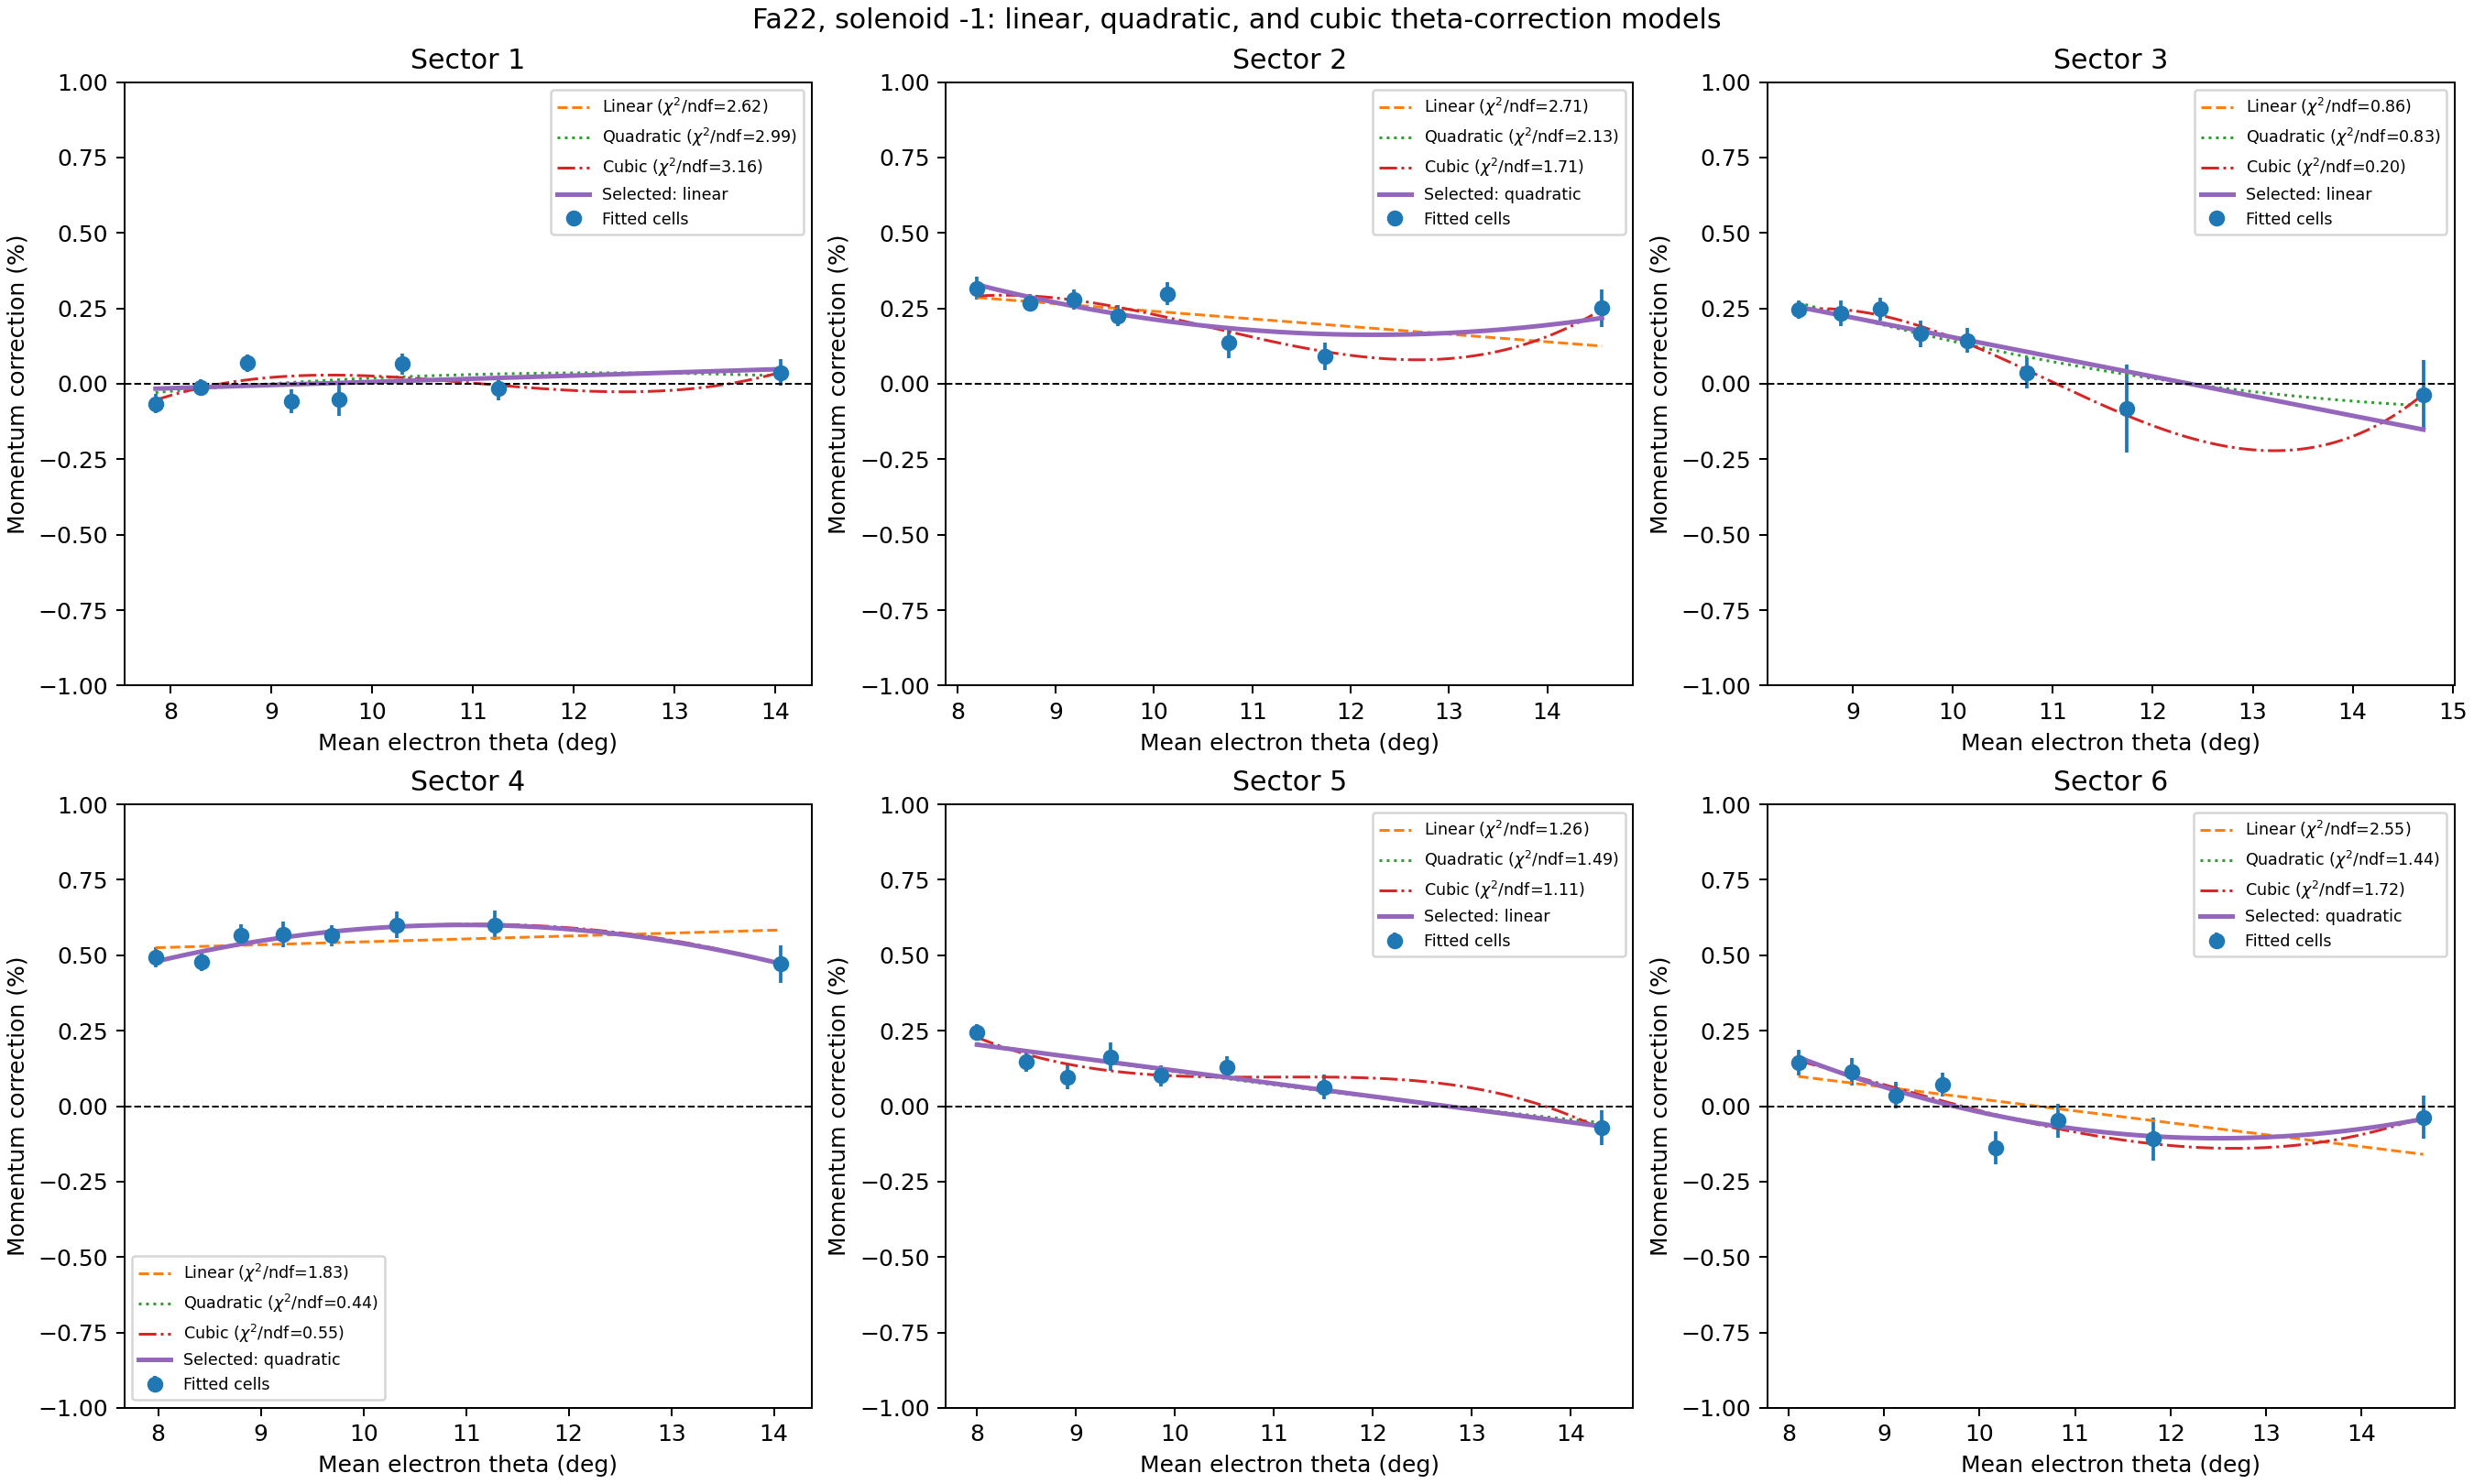
\includegraphics[width=\linewidth]{figures/channel_selection/momentum_corrections/electron/fa22_solenoid_minus_theta_model_selection.png}
\end{subfigure}
\caption{Fitted momentum correction function for the electron in each of the six FD sectors of CLAS12 as a function of $e_\theta$ for Fa22 solenoid-1.} % Caption for the whole figure
\label{fig:fa22_fitted_theta_trends}
\end{figure}

The fitted functions are presented in Tables~\ref{tab:Su22_electron_momentum_corrections}-\ref{fig:su22_integrated_before_and_after} and summary plots showing the effect of the corrections are shown in Figs.~\ref{fig:su22_integrated_before_and_after}-\ref{fig:sp23_theta_before_and_after}

\begin{table}[htbp]
\centering
\begin{tabular}{cl}
\toprule
Sector & $\delta(\theta_e)$ \\
\midrule
1 & $-0.003276 + 3.9818\times10^{-4}\theta_e$ \\
2 & $\phantom{-}0.004490 - 1.4350\times10^{-4}\theta_e$ \\
3 & $\phantom{-}0.004677 - 4.2114\times10^{-4}\theta_e$ \\
4 & $\phantom{-}0.002444 - 9.3691\times10^{-5}\theta_e$ \\
5 & $\phantom{-}0.001267 - 2.2314\times10^{-4}\theta_e$ \\
6 & $-0.001890 + 6.3591\times10^{-5}\theta_e$ \\
\bottomrule
\end{tabular}
\caption{Electron momentum correction functions for the Su22 data set. The corrected electron momentum is given by
$p_e^{\rm corr}=[1+\delta(\theta_e)]p_e$, where $\theta_e$ is in degrees. Corrections are derived for $8 < e_\theta < 15$~degrees. Tracks outside those ranges should use $\delta(8)$ or $\delta(15)$ respectively.}
\label{tab:Su22_electron_momentum_corrections}
\end{table}

\begin{table}[htbp]
\centering
\begin{tabular}{cl}
\toprule
Sector & $\delta(\theta_e)$ \\
\midrule
1 & $\phantom{-}1.9971\times10^{-4} + 1.0813\times10^{-4}\theta_e$ \\
2 & $\phantom{-}0.004853 - 1.1926\times10^{-4}\theta_e$ \\
3 & $\phantom{-}0.009825 - 6.3016\times10^{-4}\theta_e$ \\
4 & $\phantom{-}0.003173 + 2.0016\times10^{-4}\theta_e$ \\
5 & $\phantom{-}0.007813 - 6.7382\times10^{-4}\theta_e$ \\
6 & $\phantom{-}0.005404 - 4.6323\times10^{-4}\theta_e$ \\
\bottomrule
\end{tabular}
\caption{Electron momentum correction functions for the Fa22 solenoid-1 data set. Corrections are derived for $8 < e_\theta < 15$~degrees. Tracks outside those ranges should use $\delta(8)$ or $\delta(15)$ respectively.}
\label{tab:Fa22-1_electron_momentum_corrections}
\end{table}

\begin{table}[htbp]
\centering
\begin{tabular}{cl}
\toprule
Sector & $\delta(\theta_e)$ \\
\midrule
1 & $-9.8063\times10^{-4} + 1.0435\times10^{-4}\theta_e$ \\
2 & $\phantom{-}0.016937 - 0.002505\,\theta_e + 1.0245\times10^{-4}\theta_e^2$ \\
3 & $\phantom{-}0.008040 - 6.4998\times10^{-4}\theta_e$ \\
4 & $-0.010207 + 0.002954\,\theta_e - 1.3456\times10^{-4}\theta_e^2$ \\
5 & $\phantom{-}0.005466 - 4.2851\times10^{-4}\theta_e$ \\
6 & $\phantom{-}0.020615 - 0.003468\,\theta_e + 1.3870\times10^{-4}\theta_e^2$ \\
\bottomrule
\end{tabular}
\caption{Electron momentum correction functions for the Fa22 solenoid+1 data set. Corrections are derived for $8 < e_\theta < 15$~degrees. Tracks outside those ranges should use $\delta(8)$ or $\delta(15)$ respectively.}
\label{tab:Fa22+1_electron_momentum_corrections}
\end{table}

\begin{table}[htbp]
\centering
\begin{tabular}{cl}
\toprule
Sector & $\delta(\theta_e)$\\
\midrule
1 & $-0.017000 + 0.003460\,\theta_e - 1.6146\times10^{-4}\theta_e^2$ \\
2 & $\phantom{-}0.009163 - 4.5048\times10^{-4}\theta_e$ \\
3 & $\phantom{-}0.014589 - 0.001394\,\theta_e$ \\
4 & $\phantom{-}0.004071 - 3.5391\times10^{-4}\theta_e$ \\
5 & $\phantom{-}0.003038 - 5.0218\times10^{-4}\theta_e$ \\
6 & $\phantom{-}0.003121 - 3.6366\times10^{-4}\theta_e$ \\
\bottomrule
\end{tabular}
\caption{Electron momentum correction functions for the Sp23 data set. Corrections are derived for $8 < e_\theta < 15$~degrees. Tracks outside those ranges should use $\delta(8)$ or $\delta(15)$ respectively.}
\label{tab:Sp23_electron_momentum_corrections}
\end{table}  

\begin{figure}[htp]
\internallinenumbers
\begin{subfigure}[t]{0.99\textwidth}
\centering
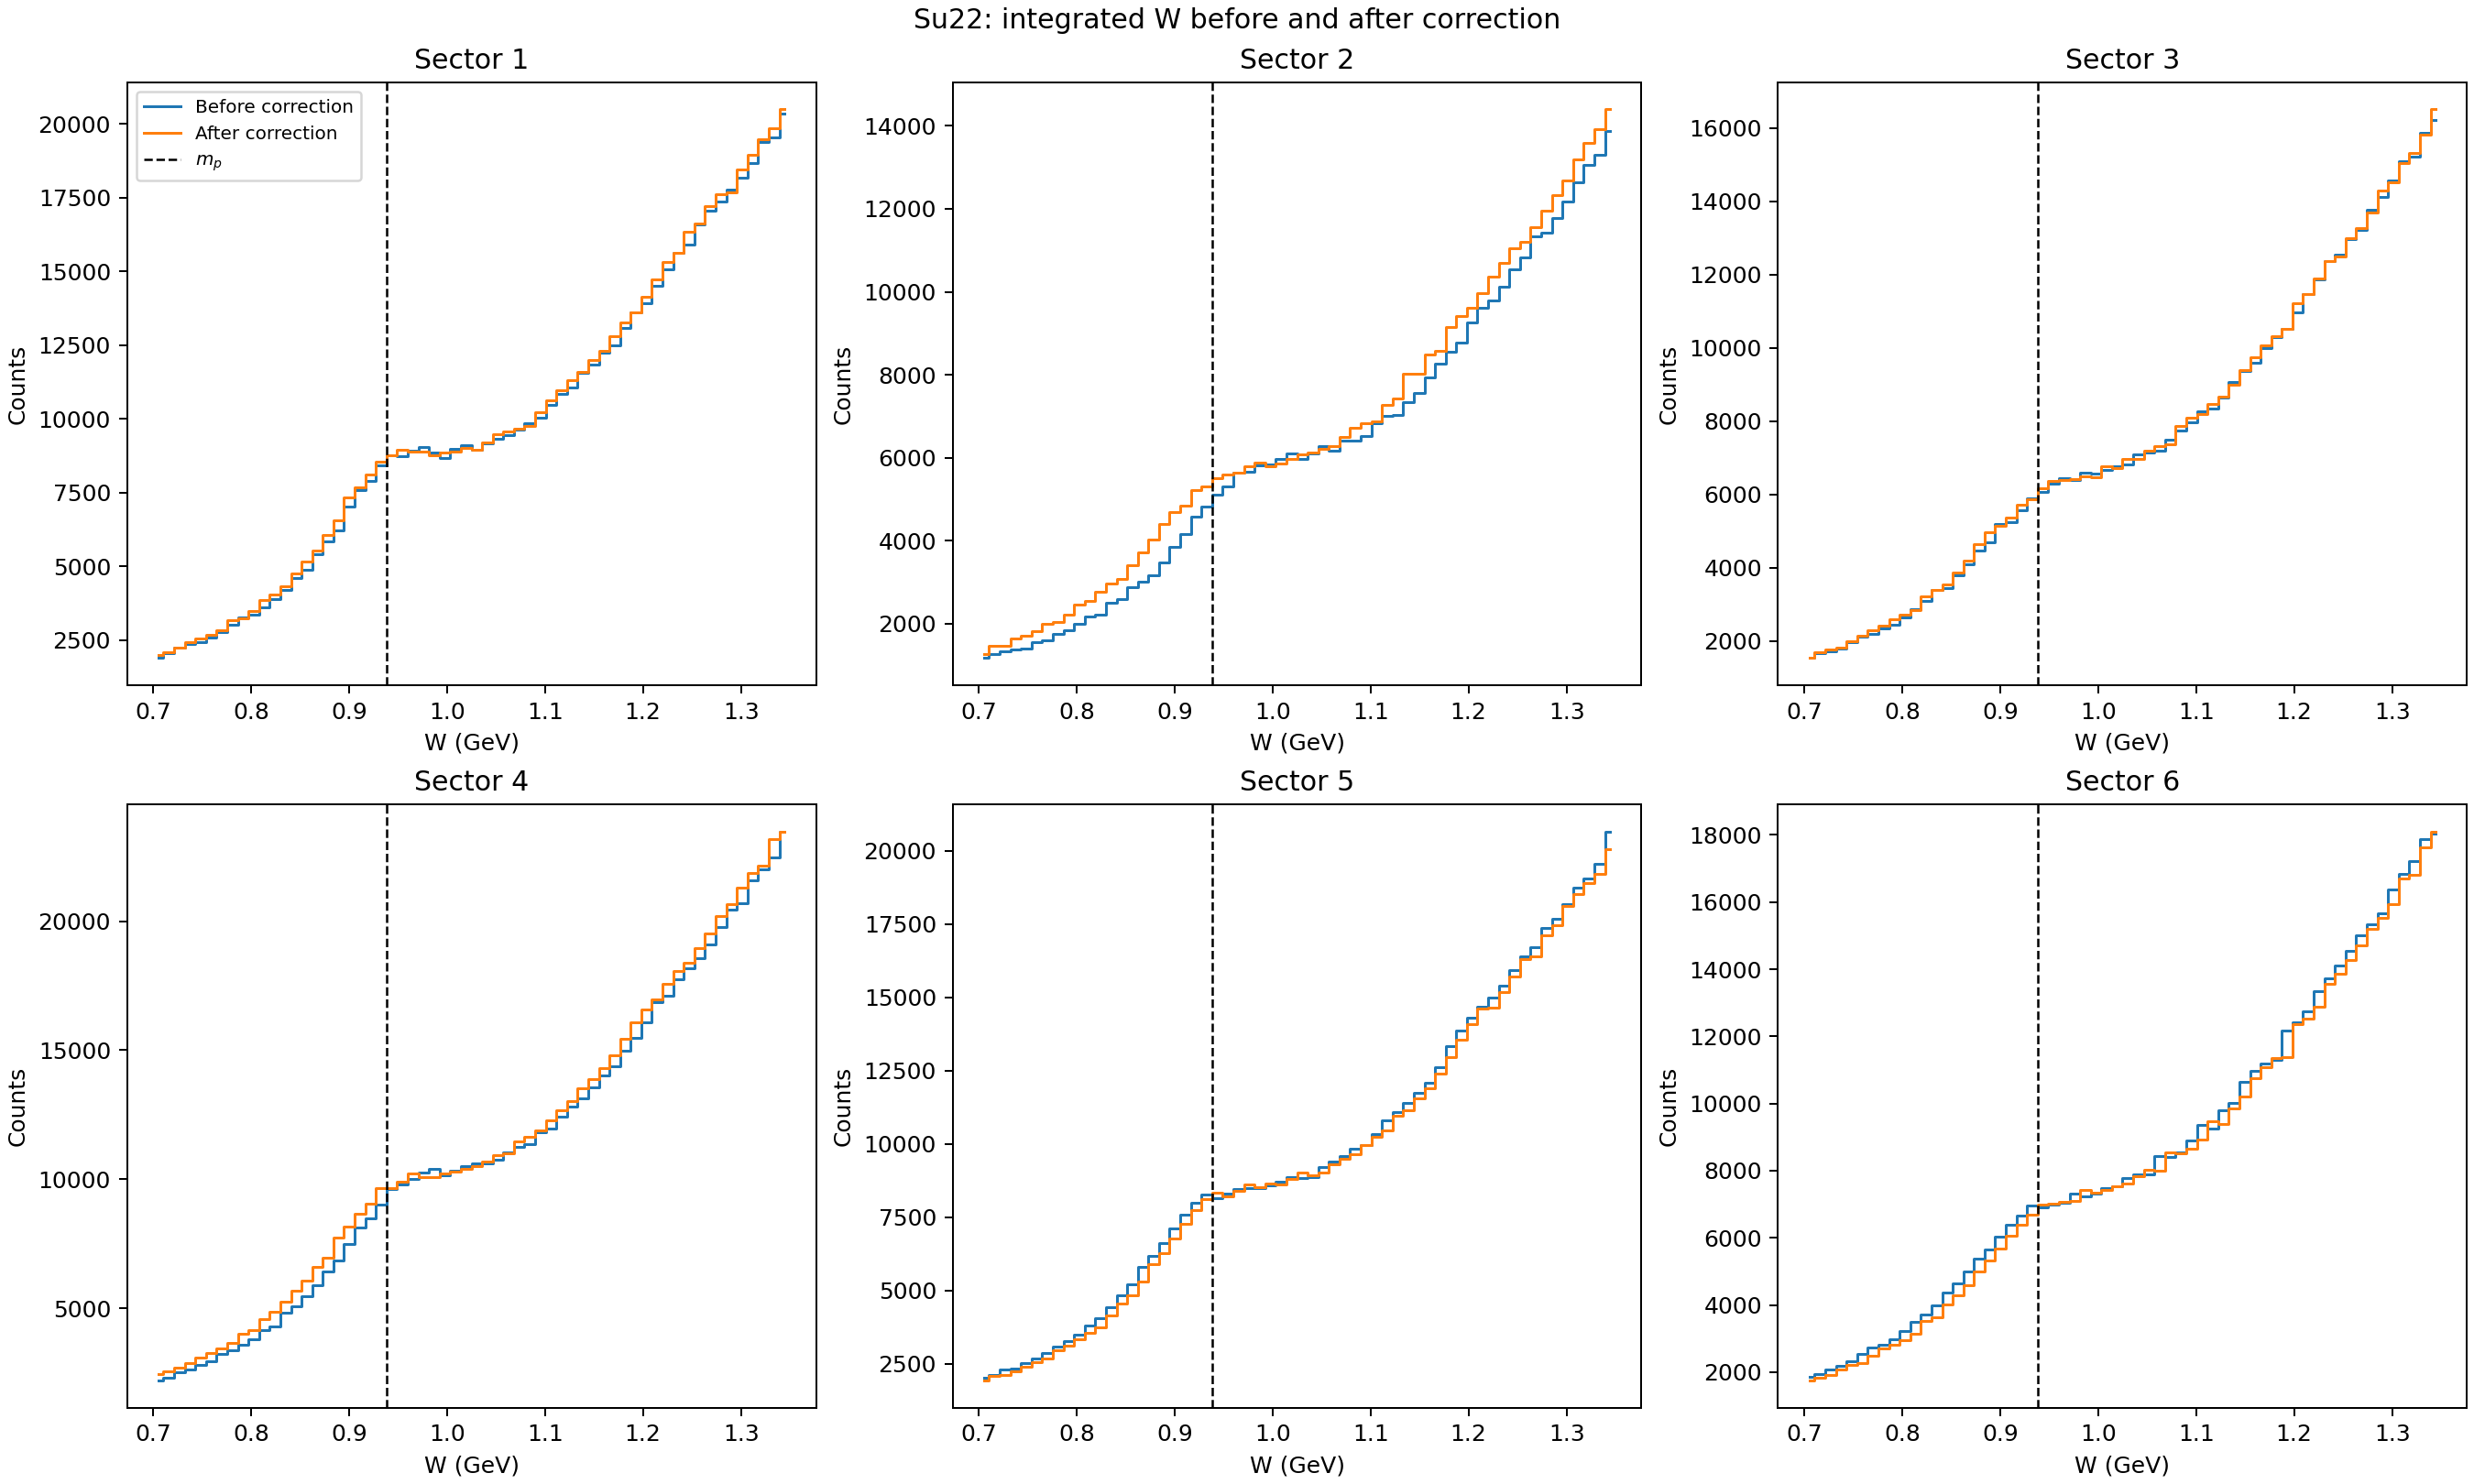
\includegraphics[width=\linewidth]{figures/channel_selection/momentum_corrections/electron/su22_integrated_w_before_after.png}
\end{subfigure}
\caption{Fitted elastic peak position before and after momentum corrections for each of the six sectors of CLAS12 for Su22.} % Caption for the whole figure
\label{fig:su22_integrated_before_and_after}
\end{figure}


\begin{figure}[htp]
\internallinenumbers
\begin{subfigure}[t]{0.99\textwidth}
\centering
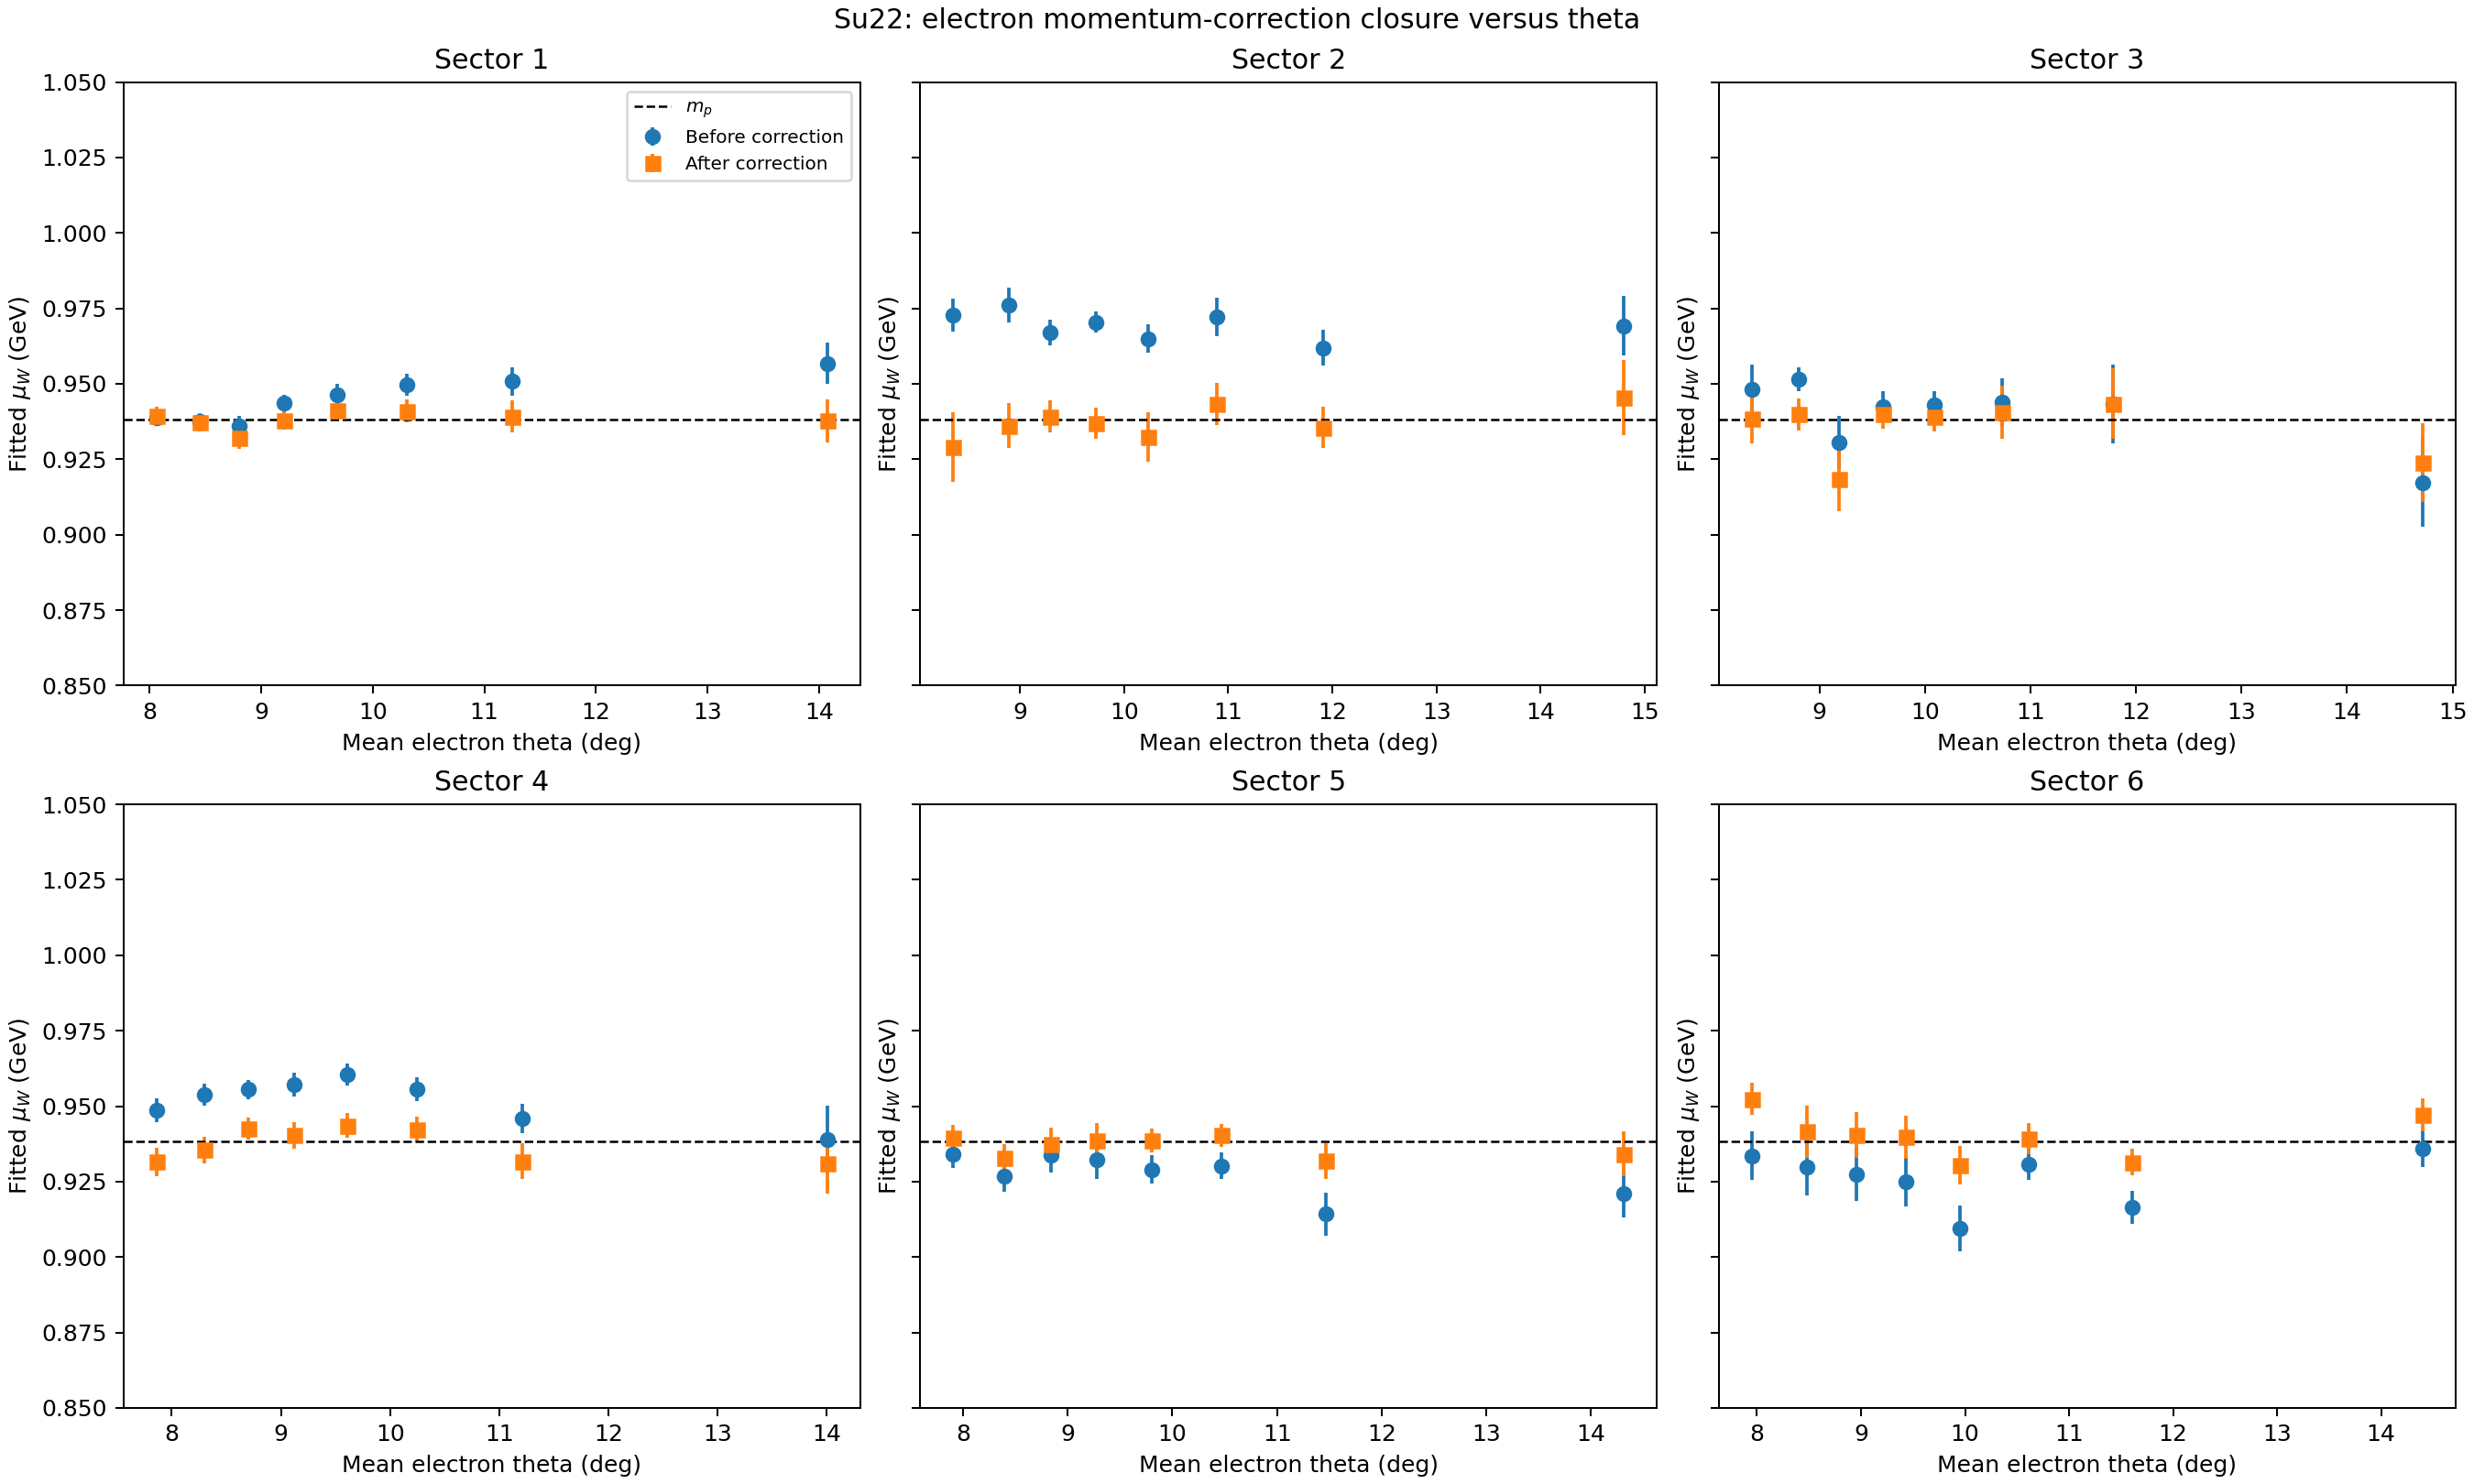
\includegraphics[width=\linewidth]{figures/channel_selection/momentum_corrections/electron/su22_theta_closure.png}
\end{subfigure}
\caption{Fitted elastic peak position before and after momentum corrections for each of the six sectors of CLAS12 for Su22 as a function of $e_\theta$} % Caption for the whole figure
\label{fig:su22_theta_before_and_after}
\end{figure}

\begin{figure}[htp]
\internallinenumbers
\begin{subfigure}[t]{0.99\textwidth}
\centering
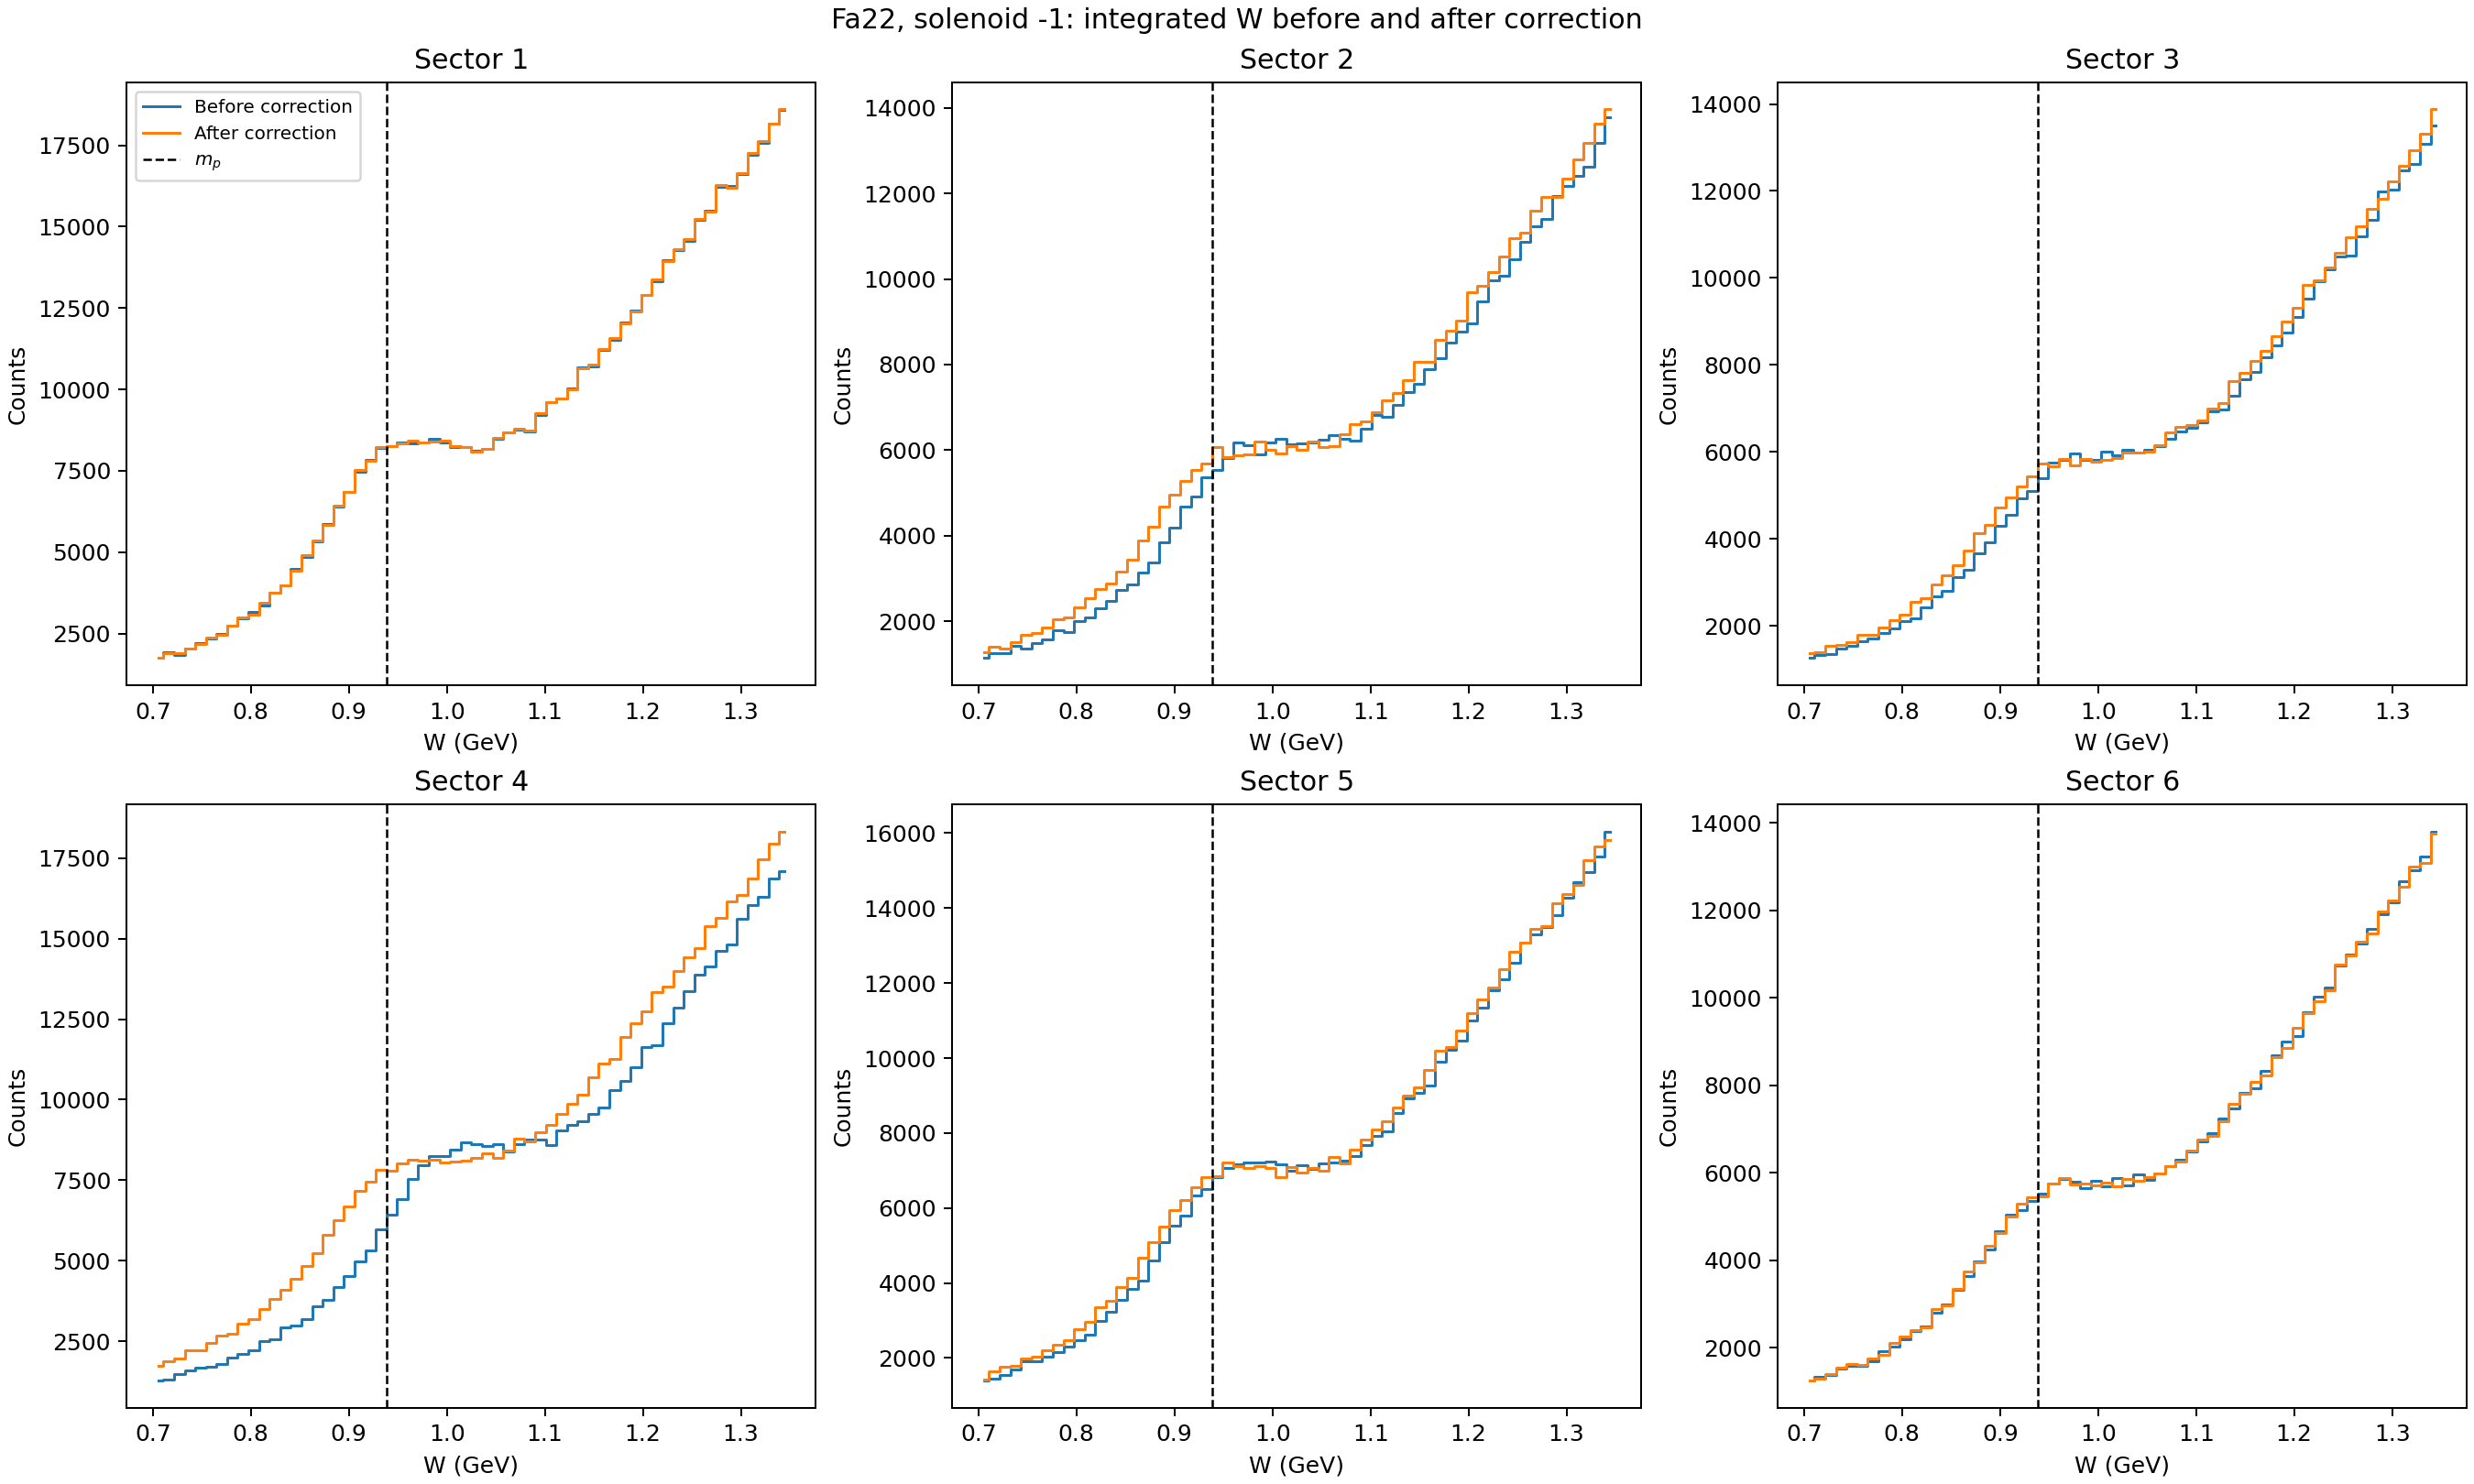
\includegraphics[width=\linewidth]{figures/channel_selection/momentum_corrections/electron/fa22_solenoid_minus_integrated_w_before_after.png}
\end{subfigure}
\caption{Fitted elastic peak position before and after momentum corrections for each of the six sectors of CLAS12 for Fa22 solenoid-1.} % Caption for the whole figure
\label{fig:fa22-1_integrated_before_and_after}
\end{figure}


\begin{figure}[htp]
\internallinenumbers
\begin{subfigure}[t]{0.99\textwidth}
\centering
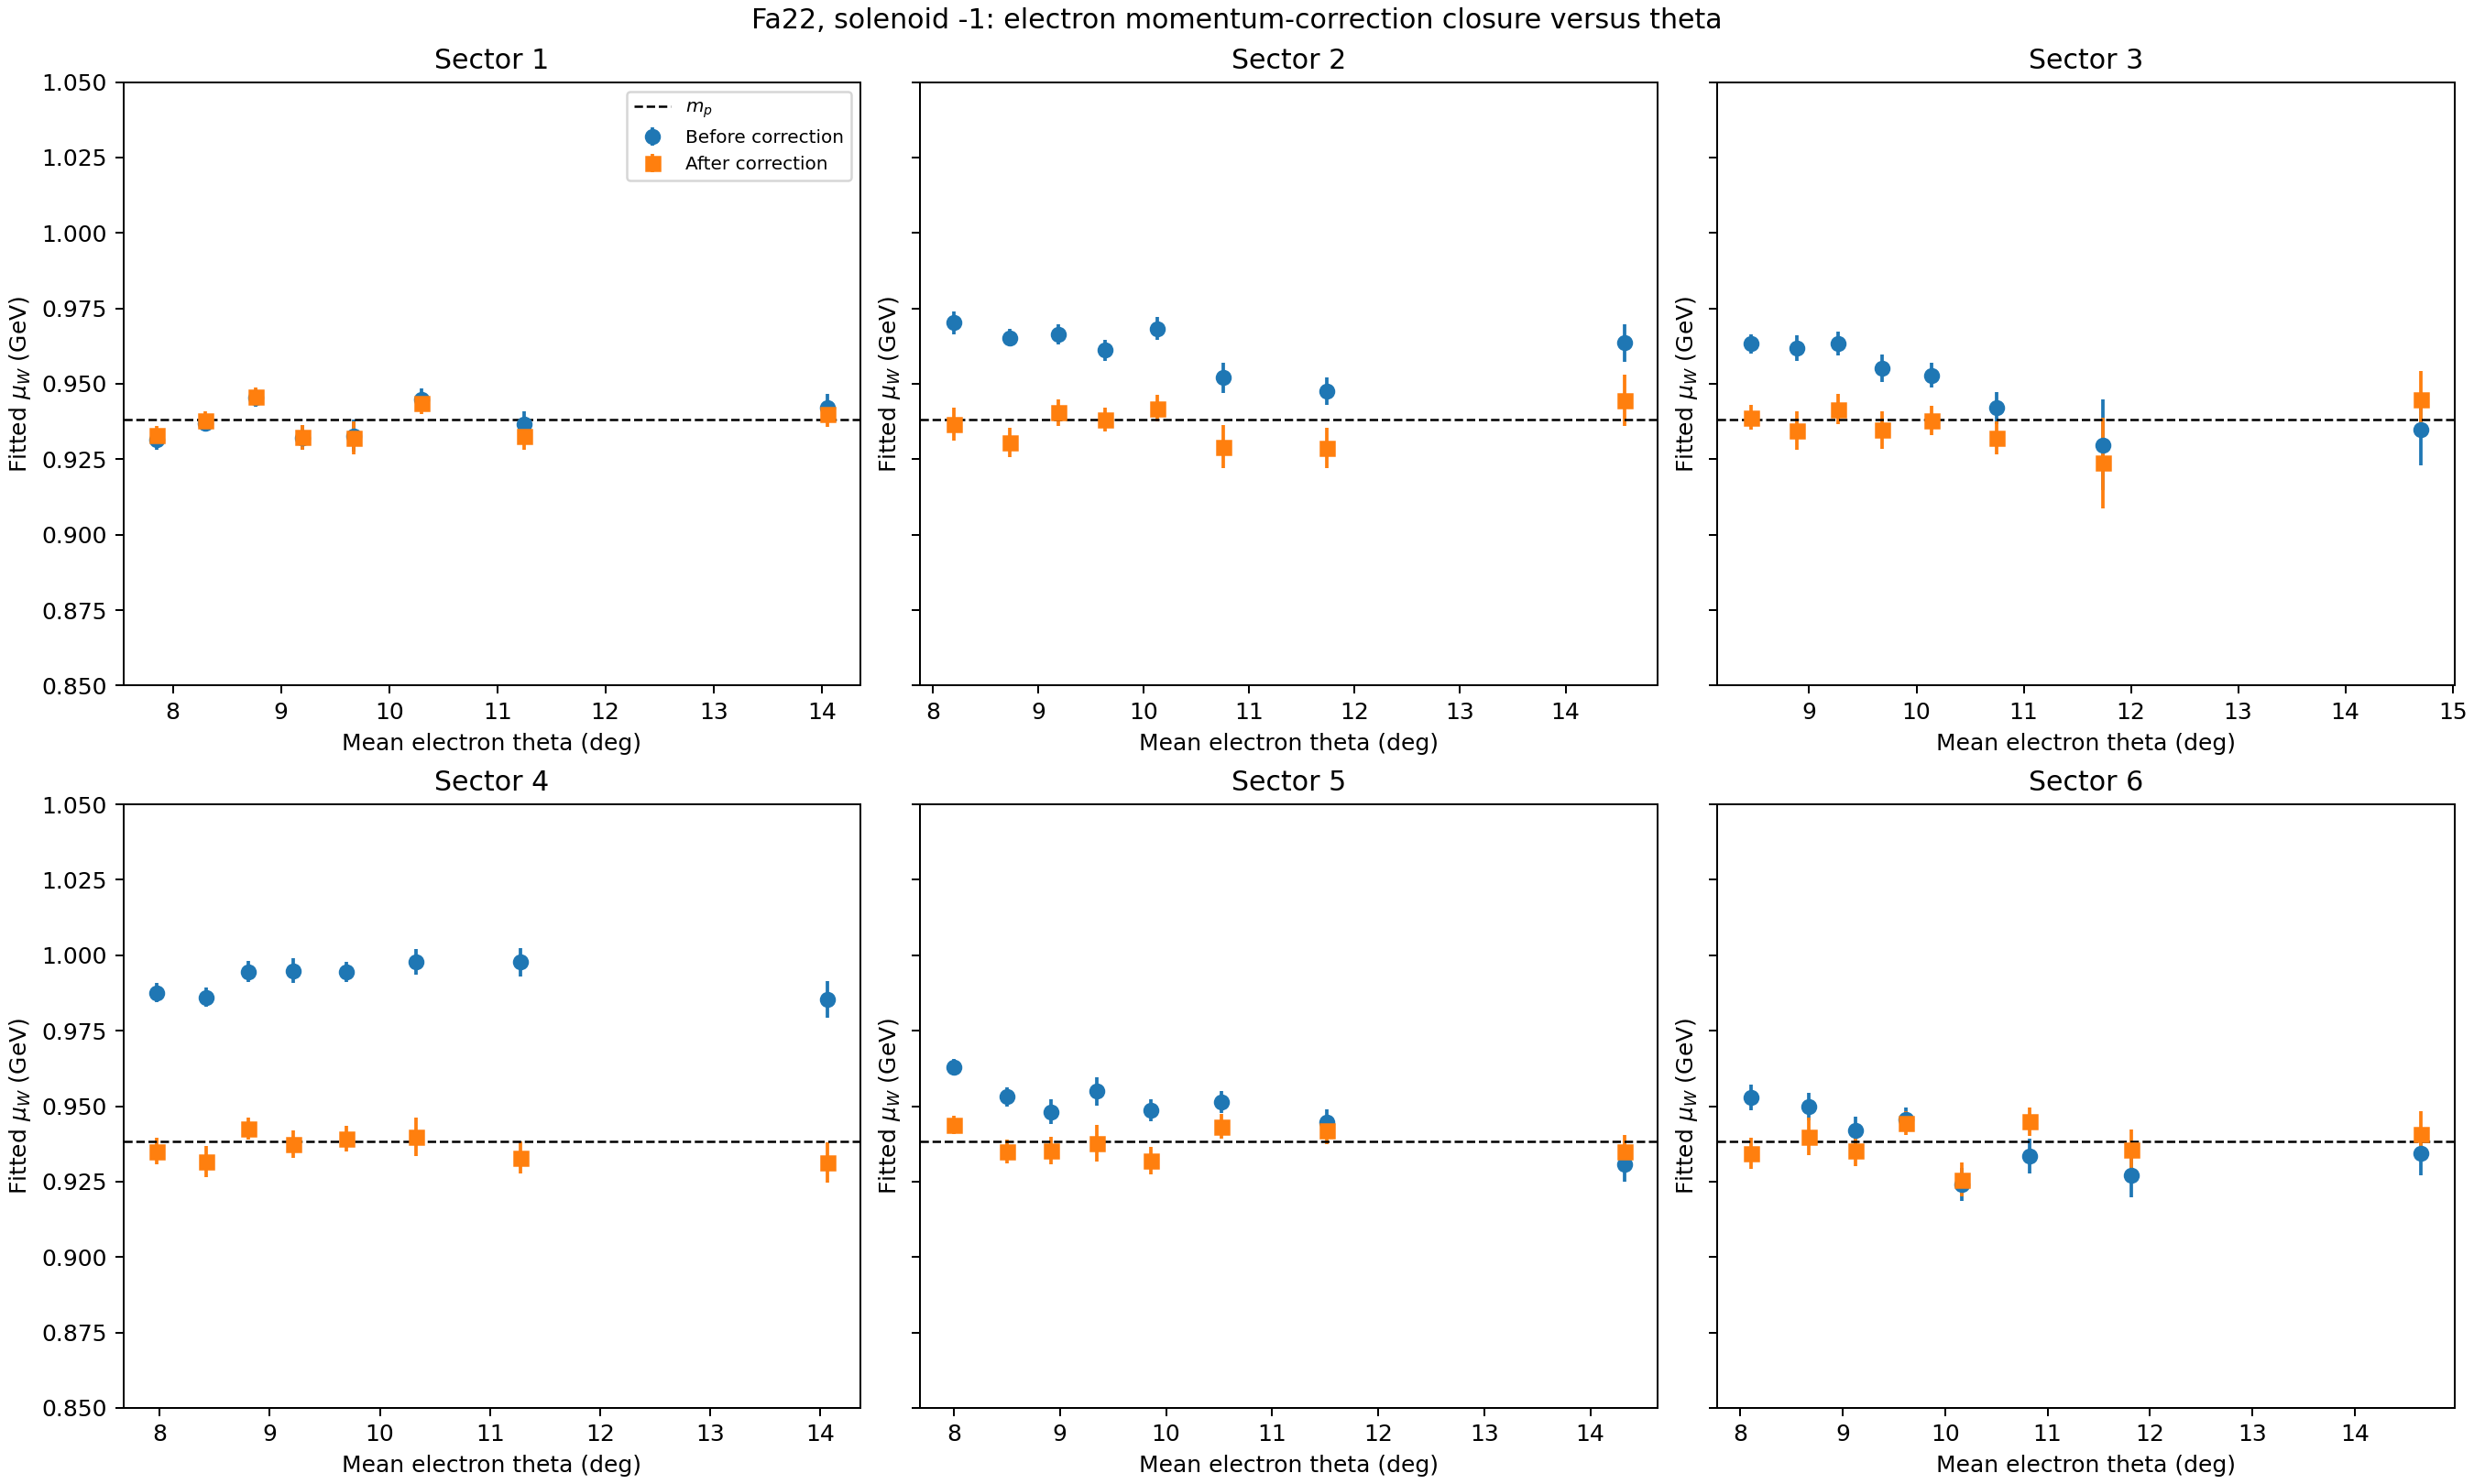
\includegraphics[width=\linewidth]{figures/channel_selection/momentum_corrections/electron/fa22_solenoid_minus_theta_closure.png}
\end{subfigure}
\caption{Fitted elastic peak position before and after momentum corrections for each of the six sectors of CLAS12 for Fa22 solenoid-1 as a function of $e_\theta$} % Caption for the whole figure
\label{fig:fa22_minus_solenoid_theta_before_and_after}
\end{figure}



\begin{figure}[htp]
\internallinenumbers
\begin{subfigure}[t]{0.99\textwidth}
\centering
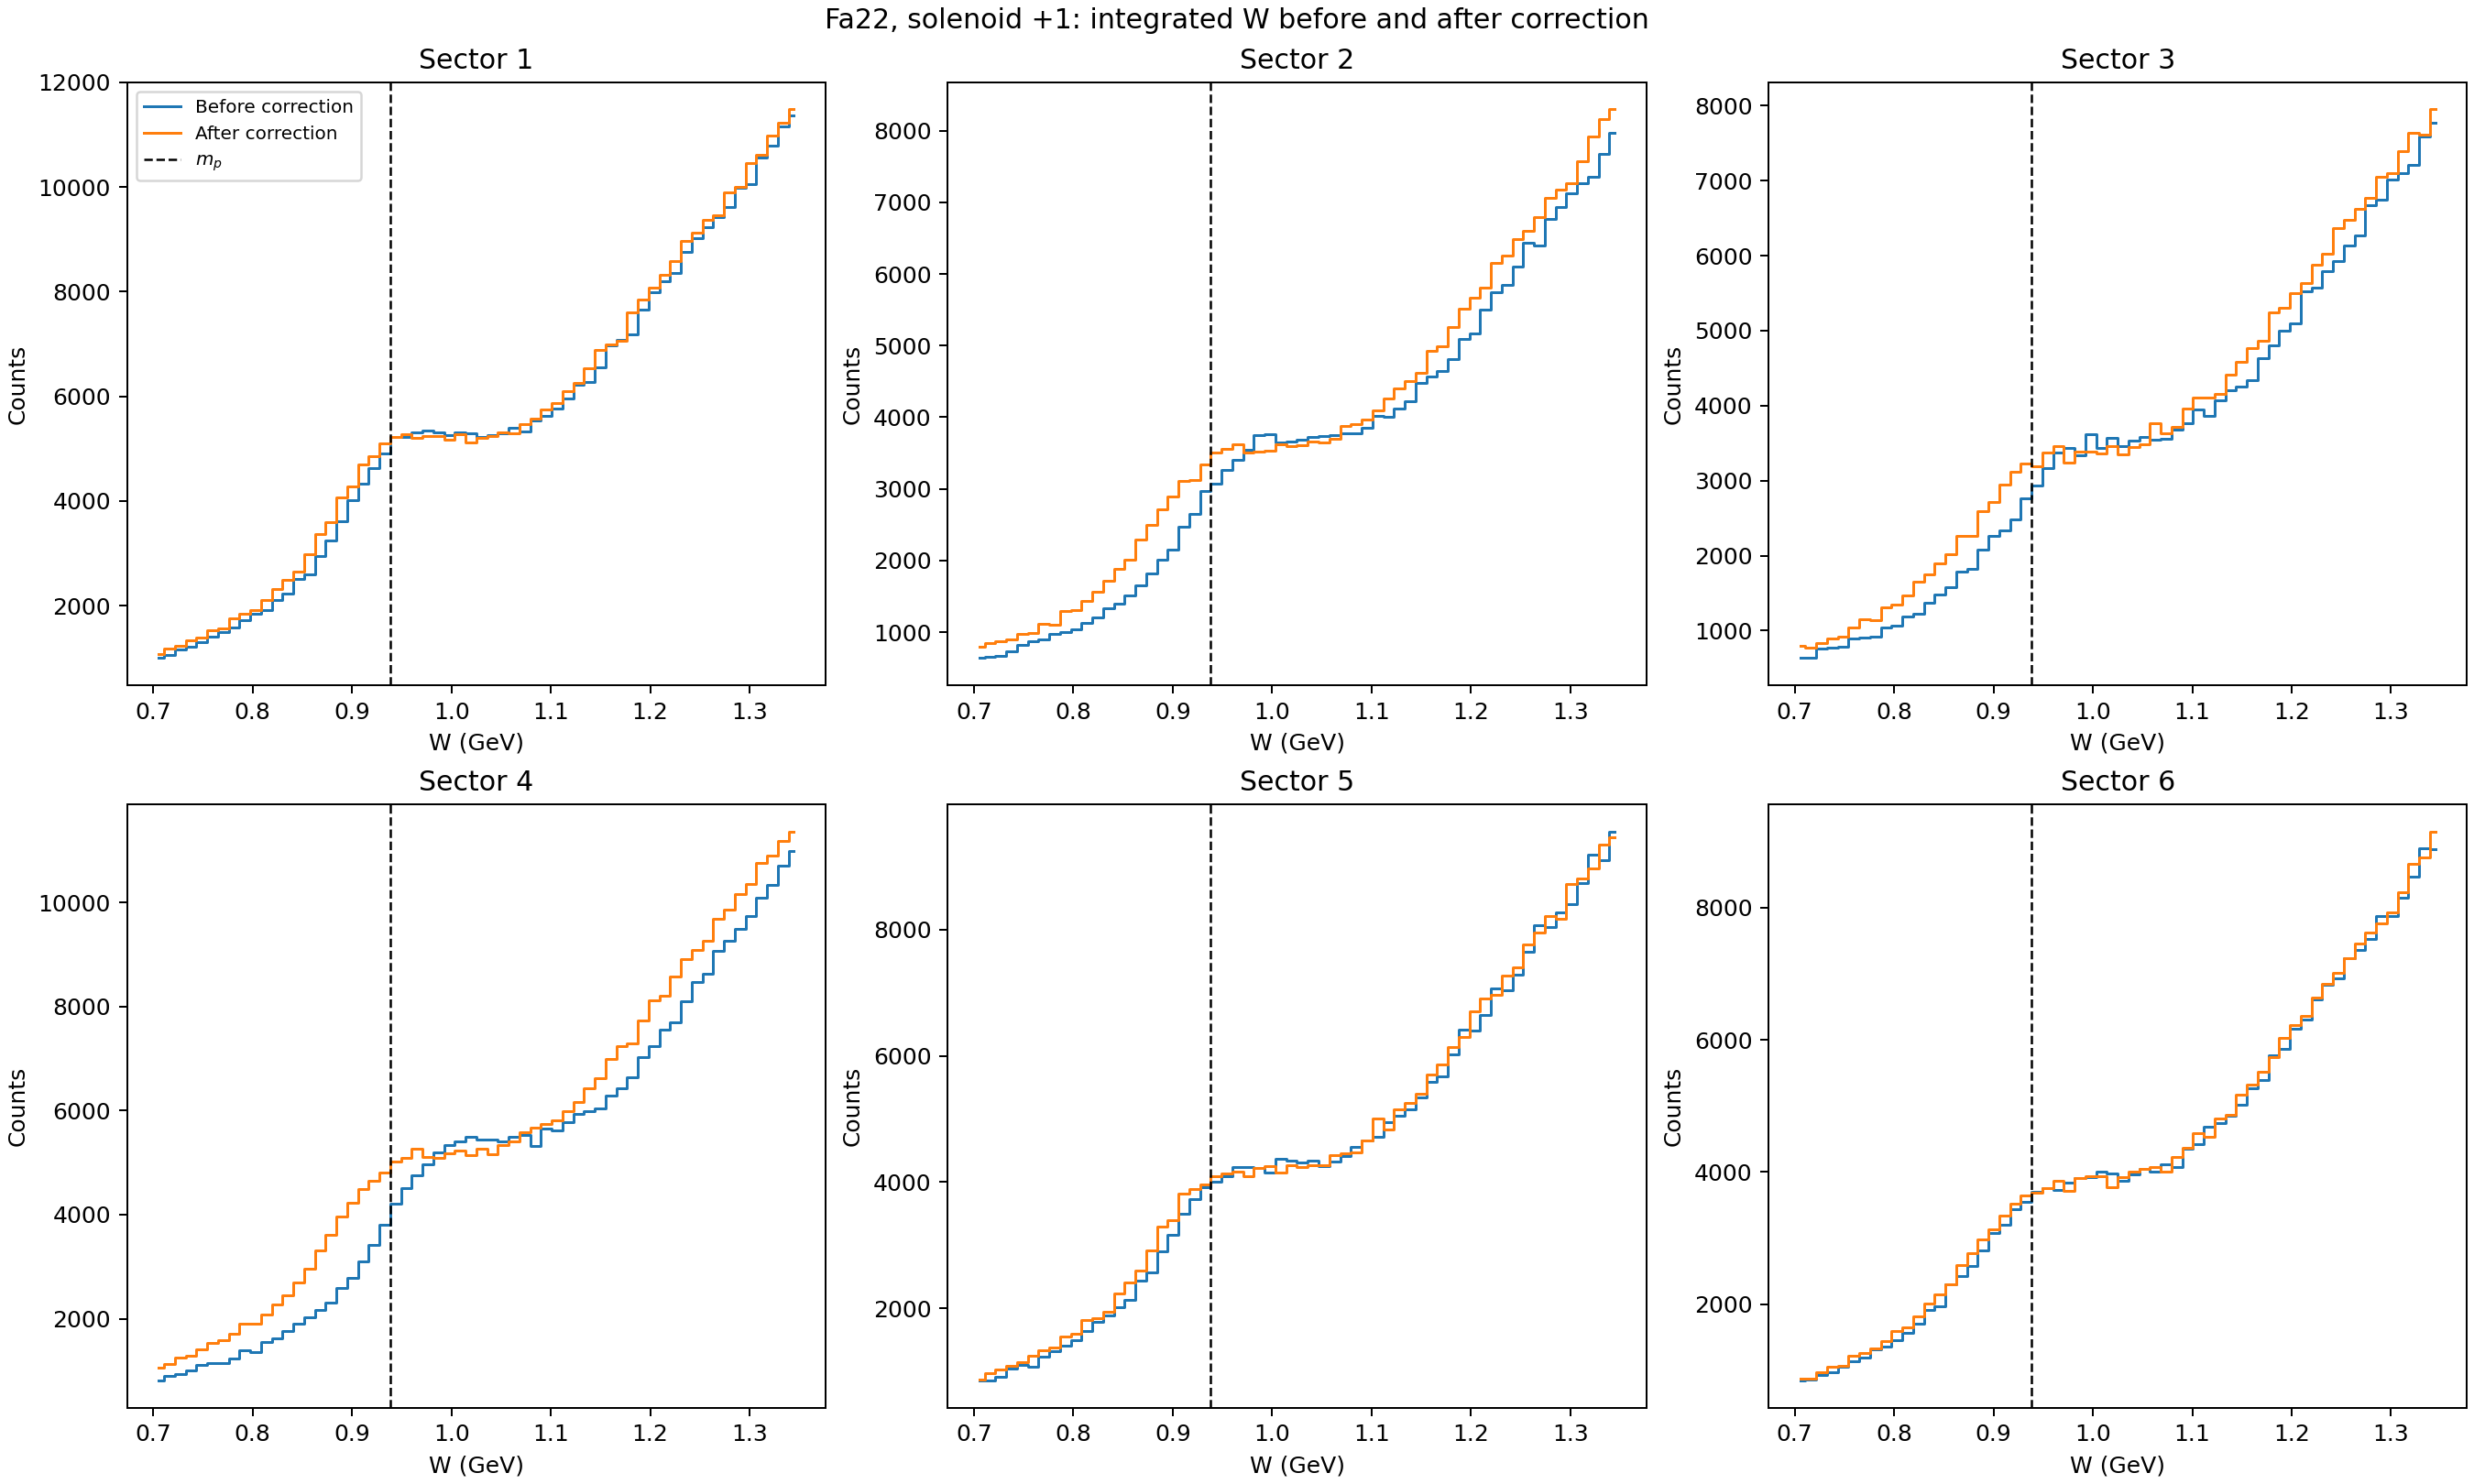
\includegraphics[width=\linewidth]{figures/channel_selection/momentum_corrections/electron/fa22_solenoid_plus_integrated_w_before_after.png}
\end{subfigure}
\caption{Fitted elastic peak position before and after momentum corrections for each of the six sectors of CLAS12 for Fa22 solenoid+1.} % Caption for the whole figure
\label{fig:fa22+1_integrated_before_and_after}
\end{figure}


\begin{figure}[htp]
\internallinenumbers
\begin{subfigure}[t]{0.99\textwidth}
\centering
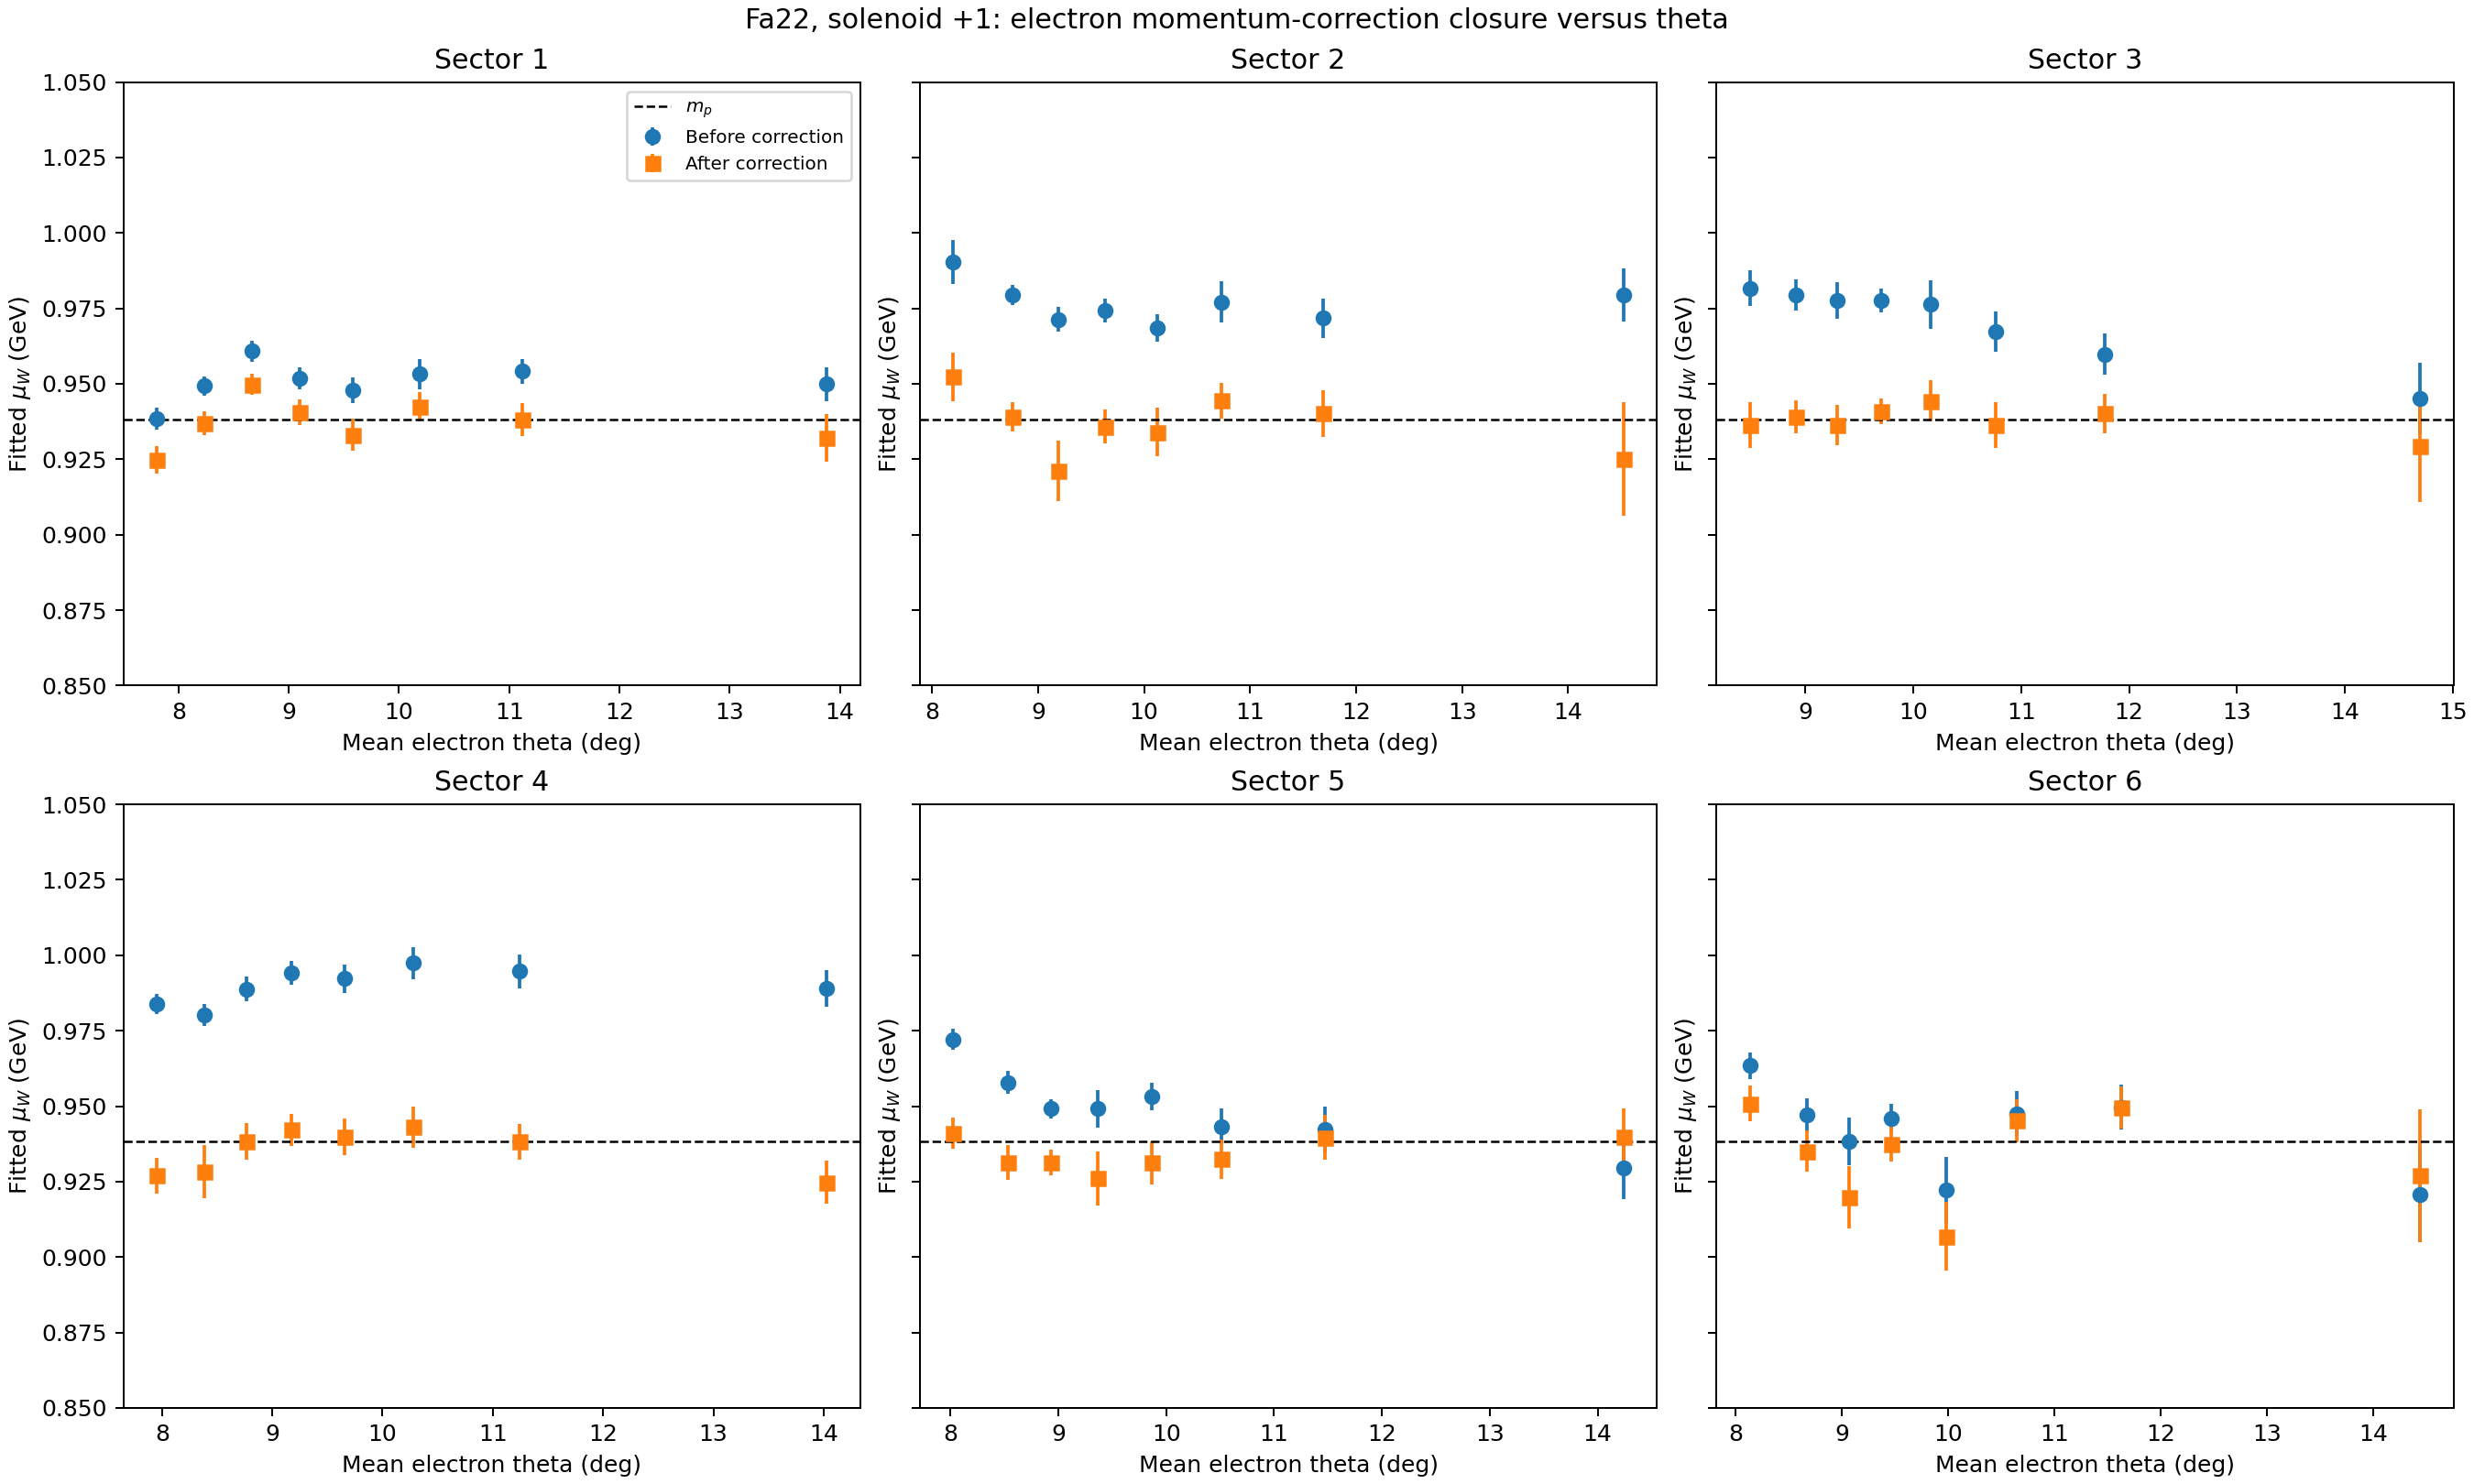
\includegraphics[width=\linewidth]{figures/channel_selection/momentum_corrections/electron/fa22_solenoid_plus_theta_closure.png}
\end{subfigure}
\caption{Fitted elastic peak position before and after momentum corrections for each of the six sectors of CLAS12 for Fa22 solenoid+1 as a function of $e_\theta$} % Caption for the whole figure
\label{fig:fa22_plus_solenoid_theta_before_and_after}
\end{figure}

\begin{figure}[htp]
\internallinenumbers
\begin{subfigure}[t]{0.99\textwidth}
\centering
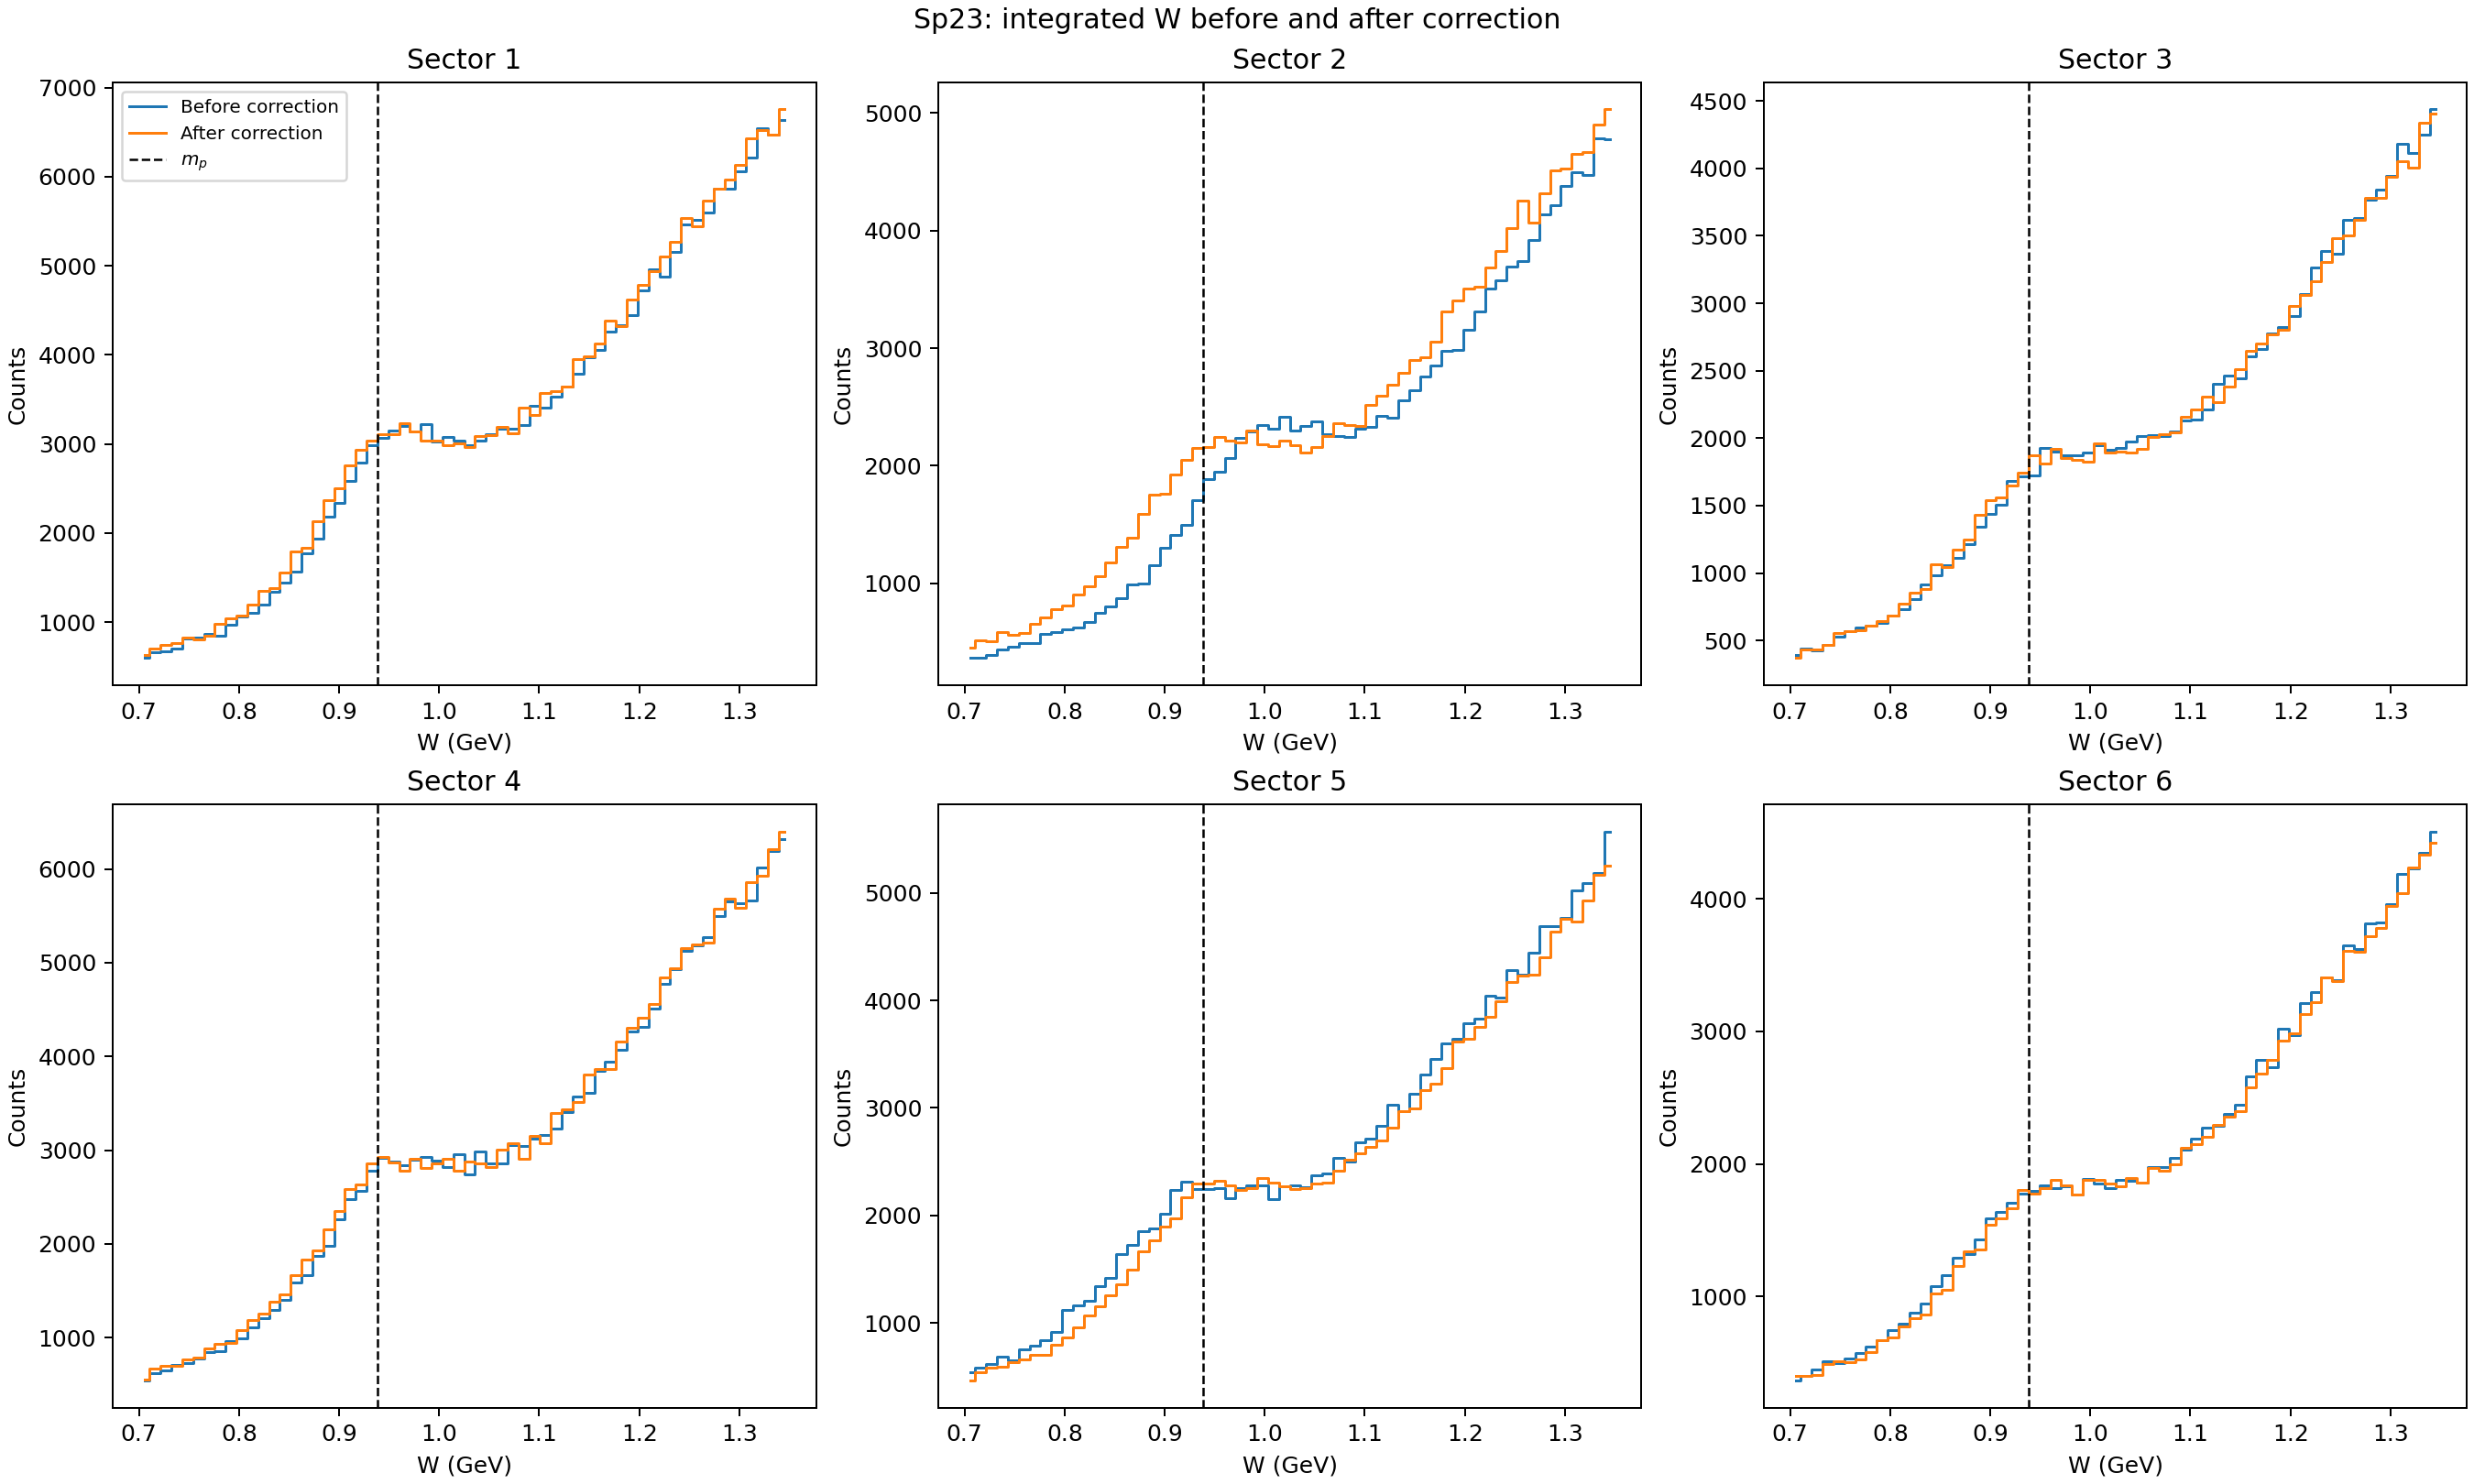
\includegraphics[width=\linewidth]{figures/channel_selection/momentum_corrections/electron/sp23_integrated_w_before_after.png}
\end{subfigure}
\caption{Fitted elastic peak position before and after momentum corrections for each of the six sectors of CLAS12 for Sp23.} % Caption for the whole figure
\label{fig:sp23_integrated_before_and_after}
\end{figure}


\begin{figure}[htp]
\internallinenumbers
\begin{subfigure}[t]{0.99\textwidth}
\centering
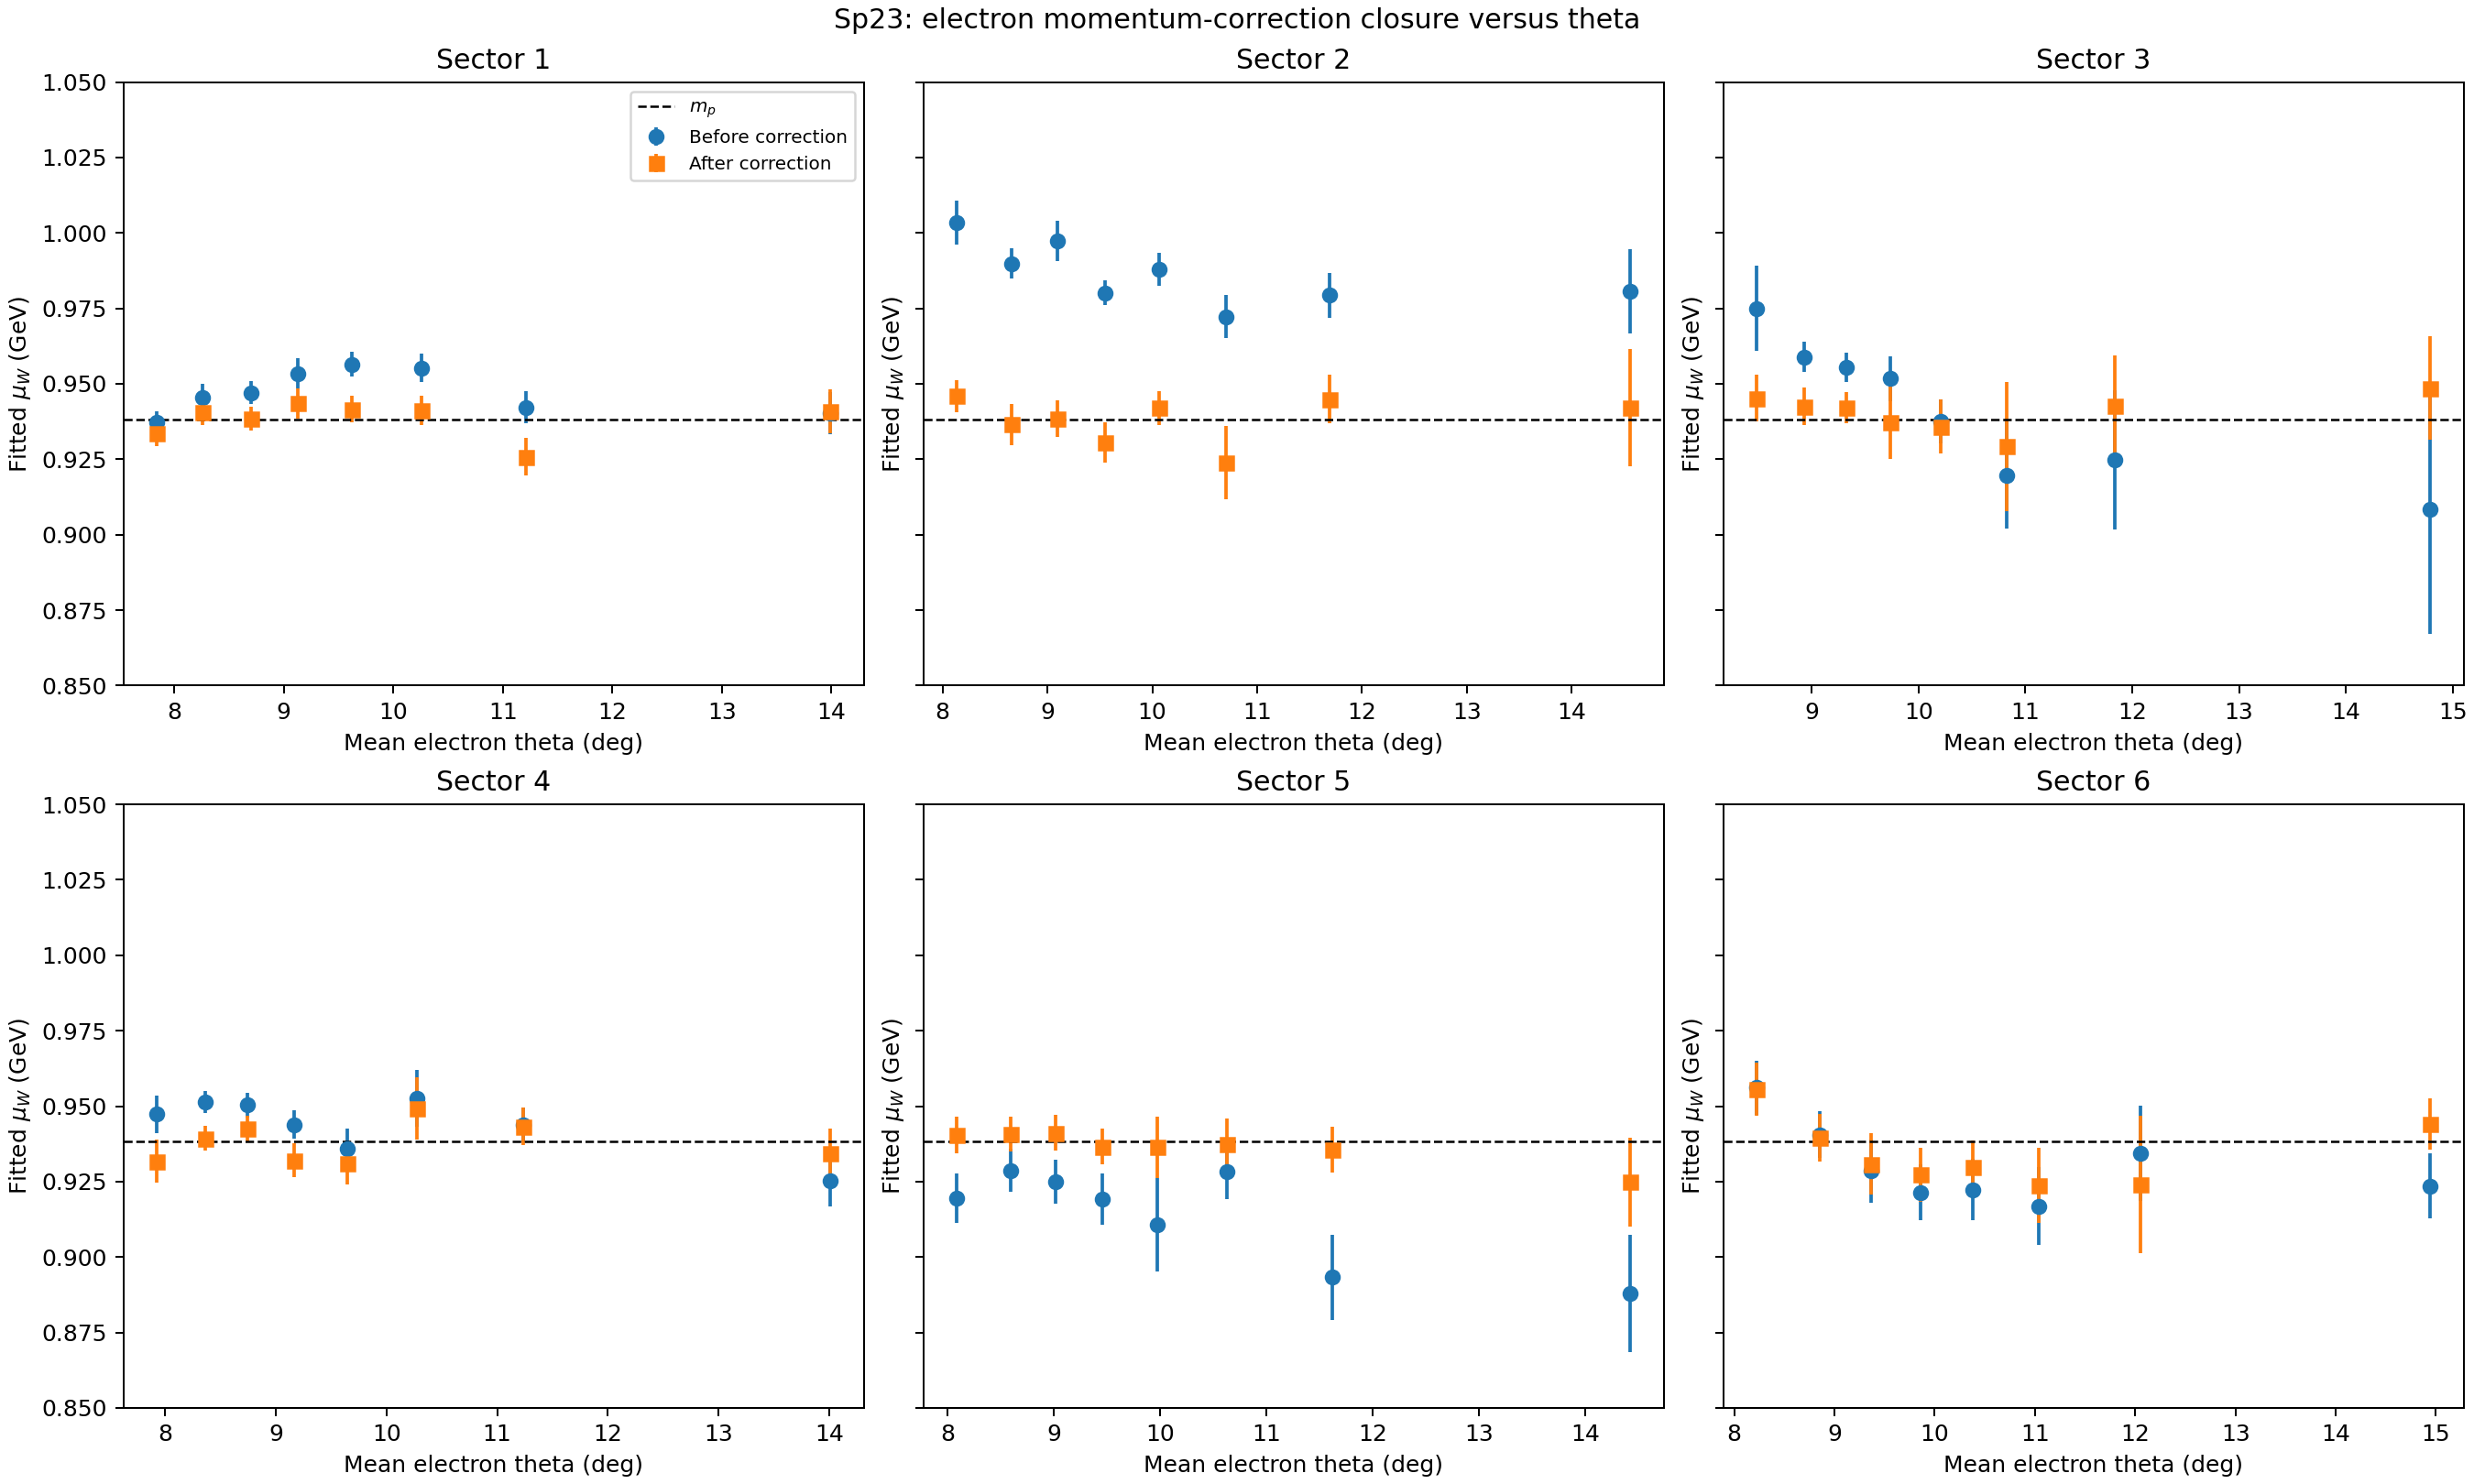
\includegraphics[width=\linewidth]{figures/channel_selection/momentum_corrections/electron/sp23_theta_closure.png}
\end{subfigure}
\caption{Fitted elastic peak position before and after momentum corrections for each of the six sectors of CLAS12 for Sp23 as a function of $e_\theta$} % Caption for the whole figure
\label{fig:sp23_theta_before_and_after}
\end{figure}

\clearpage
Only the electron momentum-correction tables above are transferred to this campaign. Their derivation/control plots are retained from the $\pi^+$ reference analysis, not presented as new ND$_3$ validation plots. The correction is $p_e^{\rm corr}=[1+\delta(\theta_e)]p_e$, with $\theta_e$ clamped to $[8,15]$ degrees and the Fa22 solenoid polarities treated separately. Corrections were also developed for $\pi^+$ in the reference analysis. Those species-specific corrections are not applied to $\pi^-$; corresponding $\pi^-$ corrections can be developed later.
